%%%%%%%%%%%%%%%%%%%%%%%%%%%%%%%%%%%%%%%%%
% The Legrand Orange Book
% LaTeX Template
% Version 2.2 (30/3/17)
%
% This template has been downloaded from:
% http://www.LaTeXTemplates.com
%
% Original author:
% Mathias Legrand (legrand.mathias@gmail.com) with modifications by:
% Vel (vel@latextemplates.com)
%
% License:
% CC BY-NC-SA 3.0 (http://creativecommons.org/licenses/by-nc-sa/3.0/)
%
% Compiling this template:
% This template uses biber for its bibliography and makeindex for its index.
% When you first open the template, compile it from the command line with the 
% commands below to make sure your LaTeX distribution is configured correctly:
%
% 1) pdflatex main
% 2) makeindex main.idx -s StyleInd.ist
% 3) biber main
% 4) pdflatex main x 2
%
% After this, when you wish to update the bibliography/index use the appropriate
% command above and make sure to compile with pdflatex several times 
% afterwards to propagate your changes to the document.
%
% This template also uses a number of packages which may need to be
% updated to the newest versions for the template to compile. It is strongly
% recommended you update your LaTeX distribution if you have any
% compilation errors.
%
% Important note:
% Chapter heading images should have a 2:1 width:height ratio,
% e.g. 920px width and 460px height.
%
%%%%%%%%%%%%%%%%%%%%%%%%%%%%%%%%%%%%%%%%%

%----------------------------------------------------------------------------------------
%	PACKAGES AND OTHER DOCUMENT CONFIGURATIONS
%----------------------------------------------------------------------------------------

\documentclass[11pt,fleqn]{book} % Default font size and left-justified equations

%----------------------------------------------------------------------------------------

%%%%%%%%%%%%%%%%%%%%%%%%%%%%%%%%%%%%%%%%%
% The Legrand Orange Book
% Structural Definitions File
% Version 2.0 (9/2/15)
%
% Original author:
% Mathias Legrand (legrand.mathias@gmail.com) with modifications by:
% Vel (vel@latextemplates.com)
% 
% This file has been downloaded from:
% http://www.LaTeXTemplates.com
%
% License:
% CC BY-NC-SA 3.0 (http://creativecommons.org/licenses/by-nc-sa/3.0/)
%
%%%%%%%%%%%%%%%%%%%%%%%%%%%%%%%%%%%%%%%%%

%----------------------------------------------------------------------------------------
%	VARIOUS REQUIRED PACKAGES AND CONFIGURATIONS
%----------------------------------------------------------------------------------------

\usepackage[top=3cm,bottom=3cm,left=3cm,right=3cm,headsep=10pt,a4paper]{geometry} % Page margins

\usepackage{graphicx} % Required for including pictures
\graphicspath{{Pictures/}} % Specifies the directory where pictures are stored

\usepackage{lipsum} % Inserts dummy text

\usepackage{tikz} % Required for drawing custom shapes

\usepackage[english]{babel} % English language/hyphenation

\usepackage{enumitem} % Customize lists
\setlist{nolistsep} % Reduce spacing between bullet points and numbered lists

\usepackage{booktabs} % Required for nicer horizontal rules in tables

\usepackage{xcolor} % Required for specifying colors by name
\definecolor{ocre}{RGB}{243,102,25} % Define the orange color used for highlighting throughout the book
\definecolor{FZJTeal}{RGB}{0,91,130}
\definecolor{FZJTan}{RGB}{238,236,225}
%----------------------------------------------------------------------------------------
%	FONTS
%----------------------------------------------------------------------------------------

\usepackage{avant} % Use the Avantgarde font for headings
%\usepackage{times} % Use the Times font for headings
\usepackage{mathptmx} % Use the Adobe Times Roman as the default text font together with math symbols from the Sym­bol, Chancery and Com­puter Modern fonts

\usepackage{microtype} % Slightly tweak font spacing for aesthetics
\usepackage[utf8]{inputenc} % Required for including letters with accents
\usepackage[T1]{fontenc} % Use 8-bit encoding that has 256 glyphs

%----------------------------------------------------------------------------------------
%	BIBLIOGRAPHY AND INDEX
%----------------------------------------------------------------------------------------

\usepackage[style=alphabetic,citestyle=numeric,sorting=nyt,sortcites=true,autopunct=true,babel=hyphen,hyperref=true,abbreviate=false,backref=true,backend=biber]{biblatex}
\addbibresource{bibliography.bib} % BibTeX bibliography file
\defbibheading{bibempty}{}

\usepackage{calc} % For simpler calculation - used for spacing the index letter headings correctly
\usepackage{makeidx} % Required to make an index
\makeindex % Tells LaTeX to create the files required for indexing

%----------------------------------------------------------------------------------------
%	MAIN TABLE OF CONTENTS
%----------------------------------------------------------------------------------------

\usepackage{titletoc} % Required for manipulating the table of contents

\contentsmargin{0cm} % Removes the default margin

% Part text styling
\titlecontents{part}[0cm]
{\addvspace{20pt}\centering\large\bfseries}
{}
{}
{}

% Chapter text styling
\titlecontents{chapter}[1.25cm] % Indentation
{\addvspace{12pt}\large\sffamily\bfseries} % Spacing and font options for chapters
{\color{FZJTeal!60}\contentslabel[\Large\thecontentslabel]{1.25cm}\color{FZJTeal}} % Chapter number
{\color{FZJTeal}}  
{\color{FZJTeal!60}\normalsize\;\titlerule*[.5pc]{.}\;\thecontentspage} % Page number

% Section text styling
\titlecontents{section}[1.25cm] % Indentation
{\addvspace{3pt}\sffamily\bfseries} % Spacing and font options for sections
{\contentslabel[\thecontentslabel]{1.25cm}} % Section number
{}
{\hfill\color{black}\thecontentspage} % Page number
[]

% Subsection text styling
\titlecontents{subsection}[1.25cm] % Indentation
{\addvspace{1pt}\sffamily\small} % Spacing and font options for subsections
{\contentslabel[\thecontentslabel]{1.25cm}} % Subsection number
{}
{\ \titlerule*[.5pc]{.}\;\thecontentspage} % Page number
[]

% List of figures
\titlecontents{figure}[0em]
{\addvspace{-5pt}\sffamily}
{\thecontentslabel\hspace*{1em}}
{}
{\ \titlerule*[.5pc]{.}\;\thecontentspage}
[]

% List of tables
\titlecontents{table}[0em]
{\addvspace{-5pt}\sffamily}
{\thecontentslabel\hspace*{1em}}
{}
{\ \titlerule*[.5pc]{.}\;\thecontentspage}
[]

%----------------------------------------------------------------------------------------
%	MINI TABLE OF CONTENTS IN PART HEADS
%----------------------------------------------------------------------------------------

% Chapter text styling
\titlecontents{lchapter}[0em] % Indenting
{\addvspace{15pt}\large\sffamily\bfseries} % Spacing and font options for chapters
{\color{FZJTeal}\contentslabel[\Large\thecontentslabel]{1.25cm}\color{FZJTeal}} % Chapter number
{}  
{\color{FZJTeal}\normalsize\sffamily\bfseries\;\titlerule*[.5pc]{.}\;\thecontentspage} % Page number

% Section text styling
\titlecontents{lsection}[0em] % Indenting
{\sffamily\small} % Spacing and font options for sections
{\contentslabel[\thecontentslabel]{1.25cm}} % Section number
{}
{}

% Subsection text styling
\titlecontents{lsubsection}[.5em] % Indentation
{\normalfont\footnotesize\sffamily} % Font settings
{}
{}
{}

%----------------------------------------------------------------------------------------
%	PAGE HEADERS
%----------------------------------------------------------------------------------------

\usepackage{fancyhdr} % Required for header and footer configuration

\pagestyle{fancy}
\renewcommand{\chaptermark}[1]{\markboth{\sffamily\normalsize\bfseries\chaptername\ \thechapter.\ #1}{}} % Chapter text font settings
\renewcommand{\sectionmark}[1]{\markright{\sffamily\normalsize\thesection\hspace{5pt}#1}{}} % Section text font settings
\fancyhf{} \fancyhead[LE,RO]{\sffamily\normalsize\thepage} % Font setting for the page number in the header
\fancyhead[LO]{\rightmark} % Print the nearest section name on the left side of odd pages
\fancyhead[RE]{\leftmark} % Print the current chapter name on the right side of even pages
\renewcommand{\headrulewidth}{0.5pt} % Width of the rule under the header
\addtolength{\headheight}{2.5pt} % Increase the spacing around the header slightly
\renewcommand{\footrulewidth}{0pt} % Removes the rule in the footer
\fancypagestyle{plain}{\fancyhead{}\renewcommand{\headrulewidth}{0pt}} % Style for when a plain pagestyle is specified

% Removes the header from odd empty pages at the end of chapters
\makeatletter
\renewcommand{\cleardoublepage}{
\clearpage\ifodd\c@page\else
\hbox{}
\vspace*{\fill}
\thispagestyle{empty}
\newpage
\fi}

%----------------------------------------------------------------------------------------
%	THEOREM STYLES
%----------------------------------------------------------------------------------------

\usepackage{amsmath,amsfonts,amssymb,amsthm} % For math equations, theorems, symbols, etc

\newcommand{\intoo}[2]{\mathopen{]}#1\,;#2\mathclose{[}}
\newcommand{\ud}{\mathop{\mathrm{{}d}}\mathopen{}}
\newcommand{\intff}[2]{\mathopen{[}#1\,;#2\mathclose{]}}
\newtheorem{notation}{Notation}[chapter]

% Boxed/framed environments
\newtheoremstyle{FZJTealnumbox}% % Theorem style name
{0pt}% Space above
{0pt}% Space below
{\normalfont}% % Body font
{}% Indent amount
{\small\bf\sffamily\color{FZJTeal}}% % Theorem head font
{\;}% Punctuation after theorem head
{0.25em}% Space after theorem head
{\small\sffamily\color{FZJTeal}\thmname{#1}\nobreakspace\thmnumber{\@ifnotempty{#1}{}\@upn{#2}}% Theorem text (e.g. Theorem 2.1)
\thmnote{\nobreakspace\the\thm@notefont\sffamily\bfseries\color{black}---\nobreakspace#3.}} % Optional theorem note
\renewcommand{\qedsymbol}{$\blacksquare$}% Optional qed square

\newtheoremstyle{blacknumex}% Theorem style name
{5pt}% Space above
{5pt}% Space below
{\normalfont}% Body font
{} % Indent amount
{\small\bf\sffamily}% Theorem head font
{\;}% Punctuation after theorem head
{0.25em}% Space after theorem head
{\small\sffamily{\tiny\ensuremath{\blacksquare}}\nobreakspace\thmname{#1}\nobreakspace\thmnumber{\@ifnotempty{#1}{}\@upn{#2}}% Theorem text (e.g. Theorem 2.1)
\thmnote{\nobreakspace\the\thm@notefont\sffamily\bfseries---\nobreakspace#3.}}% Optional theorem note

\newtheoremstyle{blacknumbox} % Theorem style name
{0pt}% Space above
{0pt}% Space below
{\normalfont}% Body font
{}% Indent amount
{\small\bf\sffamily}% Theorem head font
{\;}% Punctuation after theorem head
{0.25em}% Space after theorem head
{\small\sffamily\thmname{#1}\nobreakspace\thmnumber{\@ifnotempty{#1}{}\@upn{#2}}% Theorem text (e.g. Theorem 2.1)
\thmnote{\nobreakspace\the\thm@notefont\sffamily\bfseries---\nobreakspace#3.}}% Optional theorem note

% Non-boxed/non-framed environments
\newtheoremstyle{FZJTealnum}% % Theorem style name
{5pt}% Space above
{5pt}% Space below
{\normalfont}% % Body font
{}% Indent amount
{\small\bf\sffamily\color{FZJTeal}}% % Theorem head font
{\;}% Punctuation after theorem head
{0.25em}% Space after theorem head
{\small\sffamily\color{FZJTeal}\thmname{#1}\nobreakspace\thmnumber{\@ifnotempty{#1}{}\@upn{#2}}% Theorem text (e.g. Theorem 2.1)
\thmnote{\nobreakspace\the\thm@notefont\sffamily\bfseries\color{black}---\nobreakspace#3.}} % Optional theorem note
\renewcommand{\qedsymbol}{$\blacksquare$}% Optional qed square
\makeatother

% Defines the theorem text style for each type of theorem to one of the three styles above
\newcounter{dummy} 
\numberwithin{dummy}{section}
\theoremstyle{FZJTealnumbox}
\newtheorem{theoremeT}[dummy]{Theorem}
\newtheorem{problem}{Problem}[chapter]
\newtheorem{exerciseT}{Exercise}[chapter]
\theoremstyle{blacknumex}
\newtheorem{exampleT}{Example}[chapter]
\theoremstyle{blacknumbox}
\newtheorem{vocabulary}{Vocabulary}[chapter]
\newtheorem{definitionT}{Definition}[section]
\newtheorem{corollaryT}[dummy]{Corollary}
\theoremstyle{FZJTealnum}
\newtheorem{proposition}[dummy]{Proposition}

%----------------------------------------------------------------------------------------
%	DEFINITION OF COLORED BOXES
%----------------------------------------------------------------------------------------

\RequirePackage[framemethod=default]{mdframed} % Required for creating the theorem, definition, exercise and corollary boxes

% Theorem box
\newmdenv[skipabove=7pt,
skipbelow=7pt,
backgroundcolor=black!5,
linecolor=FZJTeal,
innerleftmargin=5pt,
innerrightmargin=5pt,
innertopmargin=5pt,
leftmargin=0cm,
rightmargin=0cm,
innerbottommargin=5pt]{tBox}

% Exercise box	  
\newmdenv[skipabove=7pt,
skipbelow=7pt,
rightline=false,
leftline=true,
topline=false,
bottomline=false,
backgroundcolor=FZJTeal!10,
linecolor=FZJTeal,
innerleftmargin=5pt,
innerrightmargin=5pt,
innertopmargin=5pt,
innerbottommargin=5pt,
leftmargin=0cm,
rightmargin=0cm,
linewidth=4pt]{eBox}	

% Definition box
\newmdenv[skipabove=7pt,
skipbelow=7pt,
rightline=false,
leftline=true,
topline=false,
bottomline=false,
linecolor=FZJTeal,
innerleftmargin=5pt,
innerrightmargin=5pt,
innertopmargin=0pt,
leftmargin=0cm,
rightmargin=0cm,
linewidth=4pt,
innerbottommargin=0pt]{dBox}	

% Corollary box
\newmdenv[skipabove=7pt,
skipbelow=7pt,
rightline=false,
leftline=true,
topline=false,
bottomline=false,
linecolor=gray,
backgroundcolor=black!5,
innerleftmargin=5pt,
innerrightmargin=5pt,
innertopmargin=5pt,
leftmargin=0cm,
rightmargin=0cm,
linewidth=4pt,
innerbottommargin=5pt]{cBox}

% Text box     
\newmdenv[skipabove=7pt,
skipbelow=7pt,
rightline=true,
leftline=true,
topline=true,
bottomline=true,
linecolor=FZJTeal,
backgroundcolor=FZJTan,
innerleftmargin=5pt,
innerrightmargin=5pt,
innertopmargin=5pt,
leftmargin=4pt,
rightmargin=4pt,
linewidth=4pt,
innerbottommargin=5pt]{fBox}

% Verbatim box 
\newmdenv[skipabove=7pt,
skipbelow=7pt,
rightline=false,
leftline=false,
topline=false,
bottomline=false,
linecolor=FZJTeal,
backgroundcolor=gray!25,
innerleftmargin=5pt,
innerrightmargin=5pt,
innertopmargin=5pt,
leftmargin=4pt,
rightmargin=4pt,
linewidth=4pt,
innerbottommargin=5pt]{VBox}
% Creates an environment for each type of theorem and assigns it a theorem text style from the "Theorem Styles" section above and a colored box from above
\newenvironment{theorem}{\begin{tBox}\begin{theoremeT}}{\end{theoremeT}\end{tBox}}
\newenvironment{exercise}{\begin{eBox}\begin{exerciseT}}{\hfill{\color{FZJTeal}\tiny\ensuremath{\blacksquare}}\end{exerciseT}\end{eBox}}				  
\newenvironment{definition}{\begin{dBox}\begin{definitionT}}{\end{definitionT}\end{dBox}}	
\newenvironment{example}{\begin{exampleT}}{\hfill{\tiny\ensuremath{\blacksquare}}\end{exampleT}}		
\newenvironment{corollary}{\begin{cBox}\begin{corollaryT}}{\end{corollaryT}\end{cBox}}	

%----------------------------------------------------------------------------------------
%	REMARK ENVIRONMENT
%----------------------------------------------------------------------------------------

\newenvironment{remark}{\par\vspace{10pt}\small % Vertical white space above the remark and smaller font size
\begin{list}{}{
\leftmargin=35pt % Indentation on the left
\rightmargin=25pt}\item\ignorespaces % Indentation on the right
\makebox[-2.5pt]{\begin{tikzpicture}[overlay]
\node[draw=FZJTeal!60,line width=1pt,circle,fill=FZJTeal!25,font=\sffamily\bfseries,inner sep=2pt,outer sep=0pt] at (-15pt,0pt){\textcolor{FZJTeal}{R}};\end{tikzpicture}} % Orange R in a circle
\advance\baselineskip -1pt}{\end{list}\vskip5pt} % Tighter line spacing and white space after remark

%----------------------------------------------------------------------------------------
%	SECTION NUMBERING IN THE MARGIN
%----------------------------------------------------------------------------------------

\makeatletter
\renewcommand{\@seccntformat}[1]{\llap{\textcolor{FZJTeal}{\csname the#1\endcsname}\hspace{1em}}}                    
\renewcommand{\section}{\@startsection{section}{1}{\z@}
{-4ex \@plus -1ex \@minus -.4ex}
{1ex \@plus.2ex }
{\normalfont\large\sffamily\bfseries}}
\renewcommand{\subsection}{\@startsection {subsection}{2}{\z@}
{-3ex \@plus -0.1ex \@minus -.4ex}
{0.5ex \@plus.2ex }
{\normalfont\sffamily\bfseries}}
\renewcommand{\subsubsection}{\@startsection {subsubsection}{3}{\z@}
{-2ex \@plus -0.1ex \@minus -.2ex}
{.2ex \@plus.2ex }
{\normalfont\small\sffamily\bfseries}}                        
\renewcommand\paragraph{\@startsection{paragraph}{4}{\z@}
{-2ex \@plus-.2ex \@minus .2ex}
{.1ex}
{\normalfont\small\sffamily\bfseries}}

%----------------------------------------------------------------------------------------
%	PART HEADINGS
%----------------------------------------------------------------------------------------

% numbered part in the table of contents
\newcommand{\@mypartnumtocformat}[2]{%
\setlength\fboxsep{0pt}%
\noindent\colorbox{FZJTeal!20}{\strut\parbox[c][.7cm]{\ecart}{\color{FZJTeal!70}\Large\sffamily\bfseries\centering#1}}\hskip\esp\colorbox{FZJTeal!40}{\strut\parbox[c][.7cm]{\linewidth-\ecart-\esp}{\Large\sffamily\centering#2}}}%
%%%%%%%%%%%%%%%%%%%%%%%%%%%%%%%%%%
% unnumbered part in the table of contents
\newcommand{\@myparttocformat}[1]{%
\setlength\fboxsep{0pt}%
\noindent\colorbox{FZJTeal!40}{\strut\parbox[c][.7cm]{\linewidth}{\Large\sffamily\centering#1}}}%
%%%%%%%%%%%%%%%%%%%%%%%%%%%%%%%%%%
\newlength\esp
\setlength\esp{4pt}
\newlength\ecart
\setlength\ecart{1.2cm-\esp}
\newcommand{\thepartimage}{}%
\newcommand{\partimage}[1]{\renewcommand{\thepartimage}{#1}}%
\def\@part[#1]#2{%
\ifnum \c@secnumdepth >-2\relax%
\refstepcounter{part}%
\addcontentsline{toc}{part}{\texorpdfstring{\protect\@mypartnumtocformat{\thepart}{#1}}{\partname~\thepart\ ---\ #1}}
\else%
\addcontentsline{toc}{part}{\texorpdfstring{\protect\@myparttocformat{#1}}{#1}}%
\fi%
\startcontents%
\markboth{}{}%
{\thispagestyle{empty}%
\begin{tikzpicture}[remember picture,overlay]%
\node at (current page.north west){\begin{tikzpicture}[remember picture,overlay]%	
\fill[FZJTeal!20](0cm,0cm) rectangle (\paperwidth,-\paperheight);
\node[anchor=north] at (4cm,-3.25cm){\color{FZJTeal!40}\fontsize{220}{100}\sffamily\bfseries\thepart}; 
\node[anchor=south east] at (\paperwidth-1cm,-\paperheight+1cm){\parbox[t][][t]{8.5cm}{
\printcontents{l}{0}{\setcounter{tocdepth}{1}}%
}};
\node[anchor=north east] at (\paperwidth-1.5cm,-3.25cm){\parbox[t][][t]{15cm}{\strut\raggedleft\color{white}\fontsize{30}{30}\sffamily\bfseries#2}};
\end{tikzpicture}};
\end{tikzpicture}}%
\@endpart}
\def\@spart#1{%
\startcontents%
\phantomsection
{\thispagestyle{empty}%
\begin{tikzpicture}[remember picture,overlay]%
\node at (current page.north west){\begin{tikzpicture}[remember picture,overlay]%	
\fill[FZJTeal!20](0cm,0cm) rectangle (\paperwidth,-\paperheight);
\node[anchor=north east] at (\paperwidth-1.5cm,-3.25cm){\parbox[t][][t]{15cm}{\strut\raggedleft\color{white}\fontsize{30}{30}\sffamily\bfseries#1}};
\end{tikzpicture}};
\end{tikzpicture}}
\addcontentsline{toc}{part}{\texorpdfstring{%
\setlength\fboxsep{0pt}%
\noindent\protect\colorbox{FZJTeal!40}{\strut\protect\parbox[c][.7cm]{\linewidth}{\Large\sffamily\protect\centering #1\quad\mbox{}}}}{#1}}%
\@endpart}
\def\@endpart{\vfil\newpage
\if@twoside
\if@openright
\null
\thispagestyle{empty}%
\newpage
\fi
\fi
\if@tempswa
\twocolumn
\fi}

%----------------------------------------------------------------------------------------
%	CHAPTER HEADINGS
%----------------------------------------------------------------------------------------

% A switch to conditionally include a picture, implemented by  Christian Hupfer
\newif\ifusechapterimage
\usechapterimagetrue
\newcommand{\thechapterimage}{}%
\newcommand{\chapterimage}[1]{\ifusechapterimage\renewcommand{\thechapterimage}{#1}\fi}%
\newcommand{\autodot}{.}
\def\@makechapterhead#1{%
{\parindent \z@ \raggedright \normalfont
\ifnum \c@secnumdepth >\m@ne
\if@mainmatter
\begin{tikzpicture}[remember picture,overlay]
\node at (current page.north west)
{\begin{tikzpicture}[remember picture,overlay]
\node[anchor=north west,inner sep=0pt] at (0,0) {\ifusechapterimage\includegraphics[width=\paperwidth]{\thechapterimage}\fi};
\draw[anchor=west] (\Gm@lmargin,-9cm) node [line width=2pt,rounded corners=15pt,draw=FZJTeal,fill=white,fill opacity=0.5,inner sep=15pt]{\strut\makebox[22cm]{}};
\draw[anchor=west] (\Gm@lmargin+.3cm,-9cm) node {\huge\sffamily\bfseries\color{black}\thechapter\autodot~#1\strut};
\end{tikzpicture}};
\end{tikzpicture}
\else
\begin{tikzpicture}[remember picture,overlay]
\node at (current page.north west)
{\begin{tikzpicture}[remember picture,overlay]
\node[anchor=north west,inner sep=0pt] at (0,0) {\ifusechapterimage\includegraphics[width=\paperwidth]{\thechapterimage}\fi};
\draw[anchor=west] (\Gm@lmargin,-9cm) node [line width=2pt,rounded corners=15pt,draw=FZJTeal,fill=white,fill opacity=0.5,inner sep=15pt]{\strut\makebox[22cm]{}};
\draw[anchor=west] (\Gm@lmargin+.3cm,-9cm) node {\huge\sffamily\bfseries\color{black}#1\strut};
\end{tikzpicture}};
\end{tikzpicture}
\fi\fi\par\vspace*{270\p@}}}

%-------------------------------------------

\def\@makeschapterhead#1{%
\begin{tikzpicture}[remember picture,overlay]
\node at (current page.north west)
{\begin{tikzpicture}[remember picture,overlay]
\node[anchor=north west,inner sep=0pt] at (0,0) {\ifusechapterimage\includegraphics[width=\paperwidth]{\thechapterimage}\fi};
\draw[anchor=west] (\Gm@lmargin,-9cm) node [line width=2pt,rounded corners=15pt,draw=FZJTeal,fill=white,fill opacity=0.5,inner sep=15pt]{\strut\makebox[22cm]{}};
\draw[anchor=west] (\Gm@lmargin+.3cm,-9cm) node {\huge\sffamily\bfseries\color{black}#1\strut};
\end{tikzpicture}};
\end{tikzpicture}
\par\vspace*{270\p@}}
\makeatother

%----------------------------------------------------------------------------------------
%	HYPERLINKS IN THE DOCUMENTS
%----------------------------------------------------------------------------------------

\usepackage{hyperref}
\hypersetup{hidelinks,backref=true,pagebackref=true,hyperindex=true,colorlinks=false,breaklinks=true,urlcolor= FZJTeal,bookmarks=true,bookmarksopen=false,pdftitle={Title},pdfauthor={Author}}
\usepackage{bookmark}
\bookmarksetup{
open,
numbered,
addtohook={%
\ifnum\bookmarkget{level}=0 % chapter
\bookmarksetup{bold}%
\fi
\ifnum\bookmarkget{level}=-1 % part
\bookmarksetup{color=FZJTeal,bold}%
\fi
}
}
 % Insert the commands.tex file which contains the majority of the structure behind the template
\newcommand{\kol}{\color{red}}
\renewcommand\Im{\operatorname{Im}}
\renewcommand\Re{\operatorname{Re}}

\begin{document}

%----------------------------------------------------------------------------------------
%	TITLE PAGE
%----------------------------------------------------------------------------------------

\begingroup
\thispagestyle{empty}
\begin{tikzpicture}[remember picture,overlay]
\node[inner sep=0pt] (background) at (current page.center) {
\includegraphics[width=\paperwidth]{background}};
\draw (current page.center) node [text=FZJTan,fill=FZJTeal!99!white,fill opacity=0.6,text opacity=1,inner sep=1cm]{\Huge\centering\bfseries\sffamily\parbox[c][][t]{\paperwidth}{\centering User Manual for KKRSUSC\\[15pt] % Book title
{\Large Linear response KKR package}\\[20pt] % Subtitle
{\Large Julen Iba\~nez, Jonathan Chico, Manuel Dos Santos \textit{et al.}}}}; % Author name
\end{tikzpicture}
\vfill
\endgroup

%----------------------------------------------------------------------------------------
%	COPYRIGHT PAGE
%----------------------------------------------------------------------------------------

\newpage
~\vfill
\thispagestyle{empty}

\noindent Copyright \copyright\ Someone \\ % Copyright notice

\noindent \textsc{Published by Publisher}\\ % Publisher

\noindent \textsc{book-website.com}\\ % URL

\noindent Licensed under License\\%Licensed under the Creative Commons Attribution-NonCommercial 3.0 Unported License (the ``License''). You may not use this file except in compliance with the License. You may obtain a copy of the License at \url{http://creativecommons.org/licenses/by-nc/3.0}. Unless required by applicable law or agreed to in writing, software distributed under the License is distributed on an \textsc{``as is'' basis, without warranties or conditions of any kind}, either express or implied. See the License for the specific language governing permissions and limitations under the License.\\ % License information

\noindent \textit{First printing, June 2017} % Printing/edition date

%----------------------------------------------------------------------------------------
%	TABLE OF CONTENTS
%----------------------------------------------------------------------------------------

%\usechapterimagefalse % If you don't want to include a chapter image, use this to toggle images off - it can be enabled later with \usechapterimagetrue

\chapterimage{ChapterImage.png} % Table of contents heading image

\pagestyle{empty} % No headers

\tableofcontents % Print the table of contents itself

\cleardoublepage % Forces the first chapter to start on an odd page so it's on the right

\pagestyle{fancy} % Print headers again

%----------------------------------------------------------------------------------------
%	PART
%----------------------------------------------------------------------------------------

\part{Part One}

%----------------------------------------------------------------------------------------
%	CHAPTER 1
%----------------------------------------------------------------------------------------

\chapterimage{ChapterImage.png} % Chapter heading image

\chapter{Prerequisites and Installation}
The \verb;KKRSUSC; program is an add-on to the main J\"ulich-M\"unich KKR \verb;JM-KKR; \textit{ab-initio} software package and its extension for impurities \verb;KKRFLEX;, that allows the calculation of dynamical properties of the system via linear response theory. The user is strongly encougraged to take some time and read the manuals and or wikis to both those packages, as a complete description of the cabailities, pitfalls and strategies for each of those programs is beyond the scope of this manual. However, basic information about each of those programs will be provided as the information that they require is necessary to be able to properly use the \verb;KKRSUSC;. 

\section{Getting the codes}\index{Getting the codes}
\label{sec:getcode}
The first step is to obtain the source code for the \verb;JM-KKR;, \verb;KKRFLEX; and \verb;KKRSUSC;. All of these software packages are available trough the \verb;IFFGit; service, to gain access to these projects contact one of the persons responsible for the code. 
\begin{fBox}
{\Large{\textbf{\sffamily\textcolor{FZJTeal}{Why Git?}}}}

Git is a very powerful version control system with an excellent web interface, allowing the users to: 
\begin{itemize}
\item Keep up to date with any changes/bugfixes in the main versions of the code.
\item Allowing for a safe development environment where changes can be reversed in case of mistakes.
\item Letting other users access the new implemented features.
\item It counts with a forum like environment for developers so that any pressing issued and or bug reports can be easily addressed by the developers.
\end{itemize}
\end{fBox}
Once access has been granted to the Git service, and the user has properly configured git in their local machine (see the Git guide provided by iffgit), the user should create a clone of the repository, for this

\begin{VBox}
\begin{verbatim}
git clone project@iffgit 
\end{verbatim}
\end{VBox}

\noindent of this way a local version of the code which is a copy of the \textbf{current} version of the code will be created. The user would then be able via the diverse git commannds (\verb;git pull;, \verb;git push; and \verb;git merge;) to update their local versions with the most recent version of the code in the repository, or to push their latest changes to the repository.

It is recommended (or is it necessary?) for the user to have the intel fortran compiler (\verb;ifort;), the MKL libraries and the intel MPI compiler. The different codes have different degrees of parallelism (Maybe ask Juba or Sascha to describe this) which can be used to accelerate the calculations.

\section{Preparation to run}\index{Preparation to run}
Before starting any calculation and or compiling any of the codes one must first see what type of calculation one wants to perform. Currently there are two types of solvers for the \verb;KKRFLEX; code and the \verb;KKRSUSC; code, whcih moostly differ in the way in which the spin orbit coupling (SOC) is terated. 

The \textit{older} version of the code, only allows the treatment of SOC as a perturbation in the \verb;KKRSUSC;. And a \textit{new} version which allows one to consider SOC all the way from the bulk calculation. Both calculations require that one setup and compile the \verb;JM-KKR; code in a different way. Hence it is very important to know which version one wants to run, for a simple guide one can take a look at Fig.~\ref{fig:CodeStruct}. 
\begin{figure}[ht]
\centering
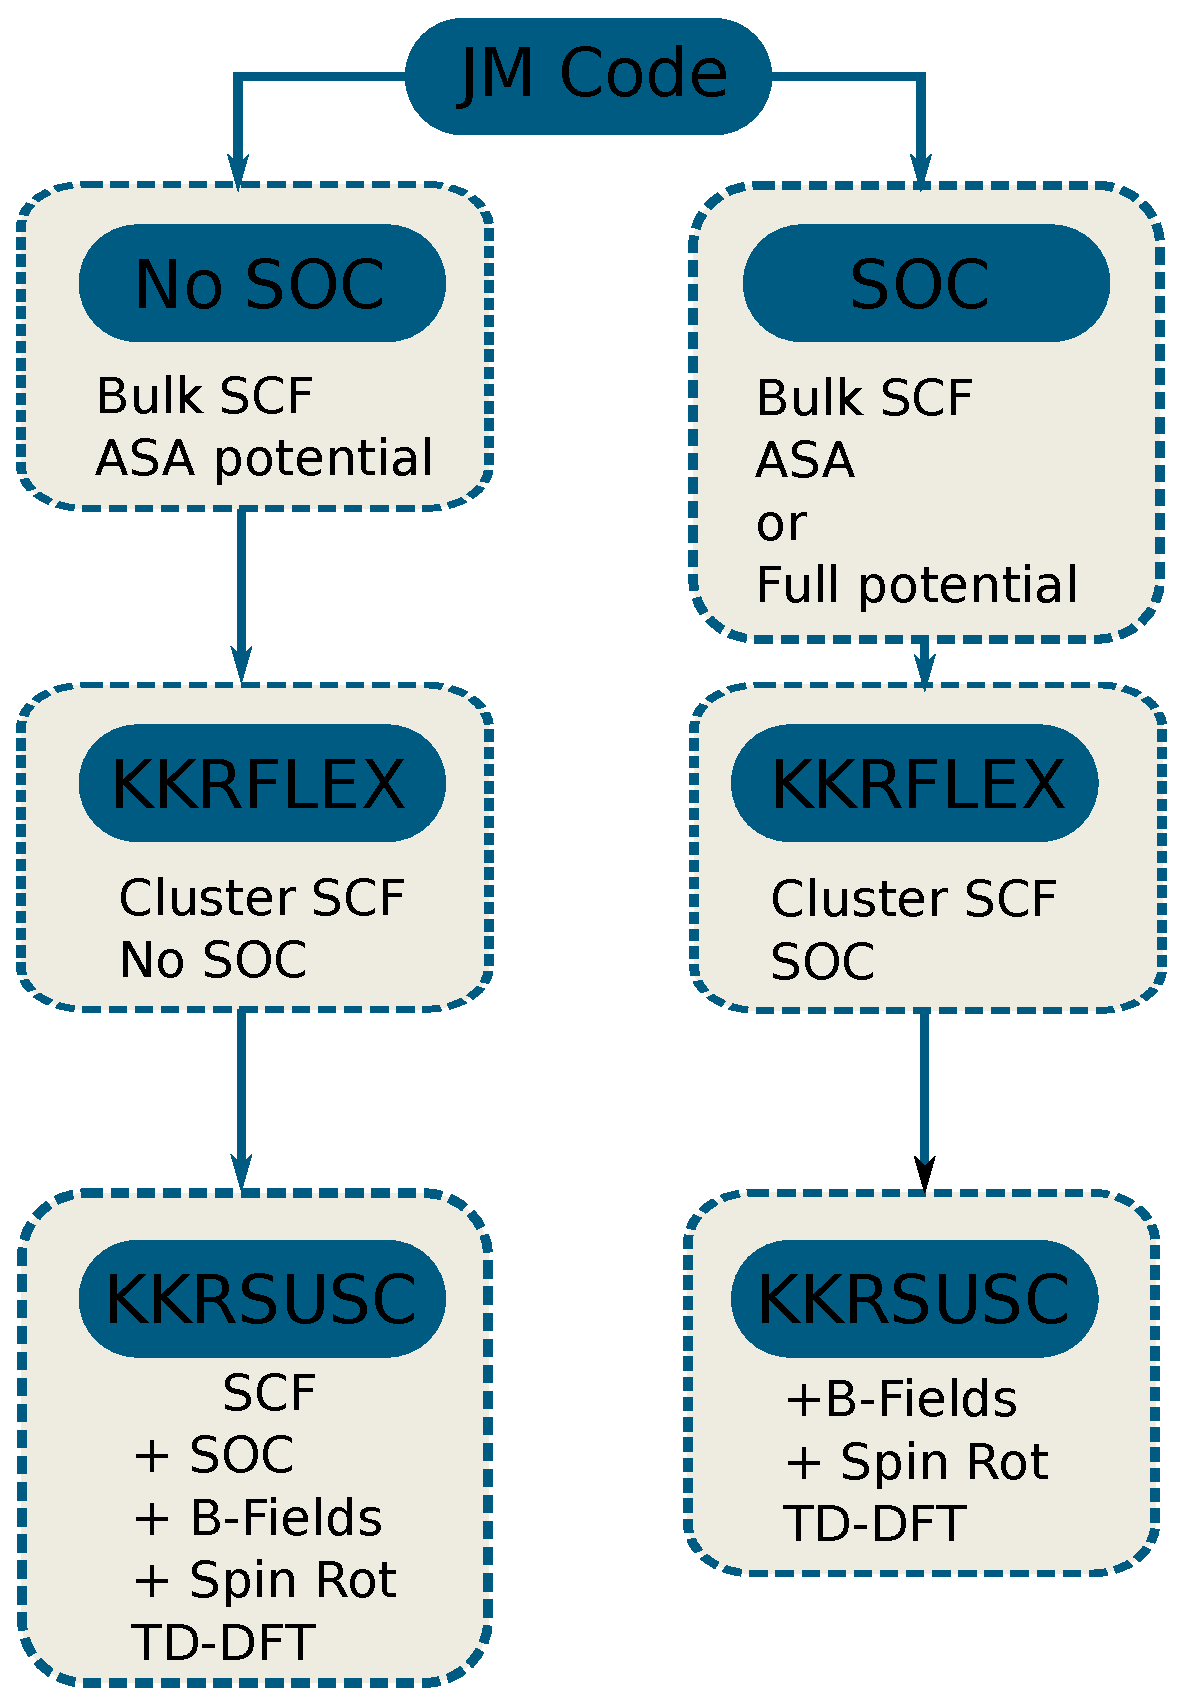
\includegraphics[width=0.75\textwidth]{./CodeStruct.eps}
\caption{Strategy for the usage of the KKR software packages to run \texttt{KKRSUSC}.\label{fig:CodeStruct}}
\end{figure}

In general the procedure to be able to run the \verb;KKRSUSC; calculation is the following, decide wheter or not one needs SOC in the host, if one does not prepare the \verb;JM-KKR; for an ASA no SOC calculation (how to do this will be explained in the next chapter), if one needs SOC in the host, prepare the \verb;JM-KKR; for a Full potential+SOC calculation. One this has been done perform an self-consitent calculation (SCF) of the potential of the host. 

After that, prepare the needed files for the \verb;KKRFLEX; (for details on that see chapter~\ref{ch:KKRFLEX}), if running with SOC use the \textit{new} solver, if not use the \textit{old} solver. Perform the SCF calculation of the cluster system that one wishes to treat. After that if SOC has been cosndiered one can then calculate the linear response funcitons that one wishes with \verb;KKRSUSC; without problem. If SOC has not been considered, run an SCF calculation+SOC in \verb;KKRSUSC; using the converged (no SOC) potential from \verb;KKRFLEX;, afterwards use that potential (\verb;KKRSUSC;+SOC SCF) to calculate the quanitites of interest via linear response.

It is important to be consistent with the approaches used (shape of the potential, inclusion of SOC) to ensure the reliability of the results. If a wrong input it given sometimes the programs will realize and will print out warnings, however, to ensure loss of time and erroneous results it falls to the user to be careful with the I/O chain from \verb;JM-KKR; all the way to \verb;KKRSUSC;.

%----------------------------------------------------------------------------------------
%	CHAPTER 2 JM-KKR
%----------------------------------------------------------------------------------------
\chapter{J\"ulich-M\"unich KKR code}\index{JM-KKR}

As mentioned in the previous chapter, to be able to perform linear response calculations in the current version of \verb;KKRSUSC; one needs to first create the appropiate files resulting from previous calculations from other KKR codes. The first one to be explored is the J\"ulich-M\"unich KKR software package (\verb;JM-KKR;). This is a firts principles calculations software package that uses the Korringa-Kohn-Rostocker (KKR)~\cite{KKR} approach to Density Functional Theory (DFT). 

\begin{fBox}
{\Large{\textbf{\sffamily\textcolor{FZJTeal}{What is KKR?}}}}

The \textbf{Kohn-Korringa-Rostocker} (KKR) method is first principles calculations method based in \textbf{Multiple Scattering Theory} (MST), and usually making use of \textbf{Green functions}, that recasts the problem of an electron interacting with an effective potential in a solid as a multiple scattering problem. 

The KKR method is often used for its capacity to make use of the \textbf{Dyson Equation}, which allows the inclusion of perturbation in a natural and simple way, thus making it a great formalism to study linear-response quantities.
\end{fBox}

This code allows for the calculation of many electronic and magnetic properties of a wide variety of systems, letting the user treat both bulk and slab structures, i.e. allowing the study of surfaces. For a full account of the capabilities of the \verb;JM-KKR; code the user is encouraged to read the user guide and manual specific for that code. If well in this guide basic user knowledge of the \verb;JM-KKR; will be given, it will be focused mostly on how it is used to generate the needed files for future calculations based on \verb;KKRFLEX; and \verb;KKRSUSC;.

\section{Compile the \texttt{JM-KKR} program}\index{Compilation}
\label{sec:compile}

Before compiling the \verb;JM-KKR; code one must think about the type of system that one wants to simulate. This is because there are a set of arrays in the code with fixed lenght, which depend on the properties of the system. Some of the most common quantities that will-force the user to re-compile the code are the following:
\begin{itemize}
\item ASA or FP calculation. \verb;KSHAPE;
\item SOC or no SOC in the host. \verb;KORBIT;
\item Number of atoms in the unit cell. \verb;NAEZD;
\item Magnetic/non-magnetic host calculation. \verb;KSP;
\item Number of principal layers needed. \verb;NPRINCD;
\item Maximum value of the expansion for the angular momentum. \verb;LMAXD;
\end{itemize} 

As can be seen each of these variables has a well defined keyword, these can be found in a filne named \verb;inc.p; which is found in the source folder of the \verb;JM-KKR; code. If one is going to perform a calculation that requires one to change one or more of these variables \textbf{one must re-compile the code}. 

After one has looked into the inc.p file and has made sure that all the variables presented there have the correct variables one must compile the code, to do that one must do the following in the source folder

\begin{itemize}
\item To compile the serial version:
\begin{VBox}
\begin{verbatim}
make all
\end{verbatim}
\end{VBox}
\item To compile the parallel version:
\begin{VBox}
\begin{verbatim}
make allmpi
\end{verbatim}
\end{VBox}
\item To clean:
\begin{VBox}
\begin{verbatim}
make clean
\end{verbatim}
\end{VBox}
 \end{itemize}
\begin{fBox}

{\Large{\textbf{\sffamily\textcolor{FZJTeal}{Tip: Always be saving}}}}

One would probably need to run several simulations with the same number of atoms, magnetic/or non-magnetic host, shape of the potential, etc. Hence, it is a good idea to create a folder for each set of variables, where one can store both the executable \verb;kkr.x; and the \verb;inc.p; file. Of this way these files can be re-used and one would just need to modify the \textit{flexible} variables in the input file of the code.

\end{fBox} 

After saving the \verb;inc.p; and the \verb;kkr.x; files in the folders the code is ready to run. It is important to notice that there are many versions of the code, and the methods described here are valid for the \textit{current} version of the code, i.e. any version from at least 05-01-2017. 

\subsection{Brief list of what each executable does for \textit{legacy} versions of \texttt{JM-KKR}}
\label{sec:executables}

In this version the \verb;JM-KKR; has only one executable for the SCF run, however, there are some other versions of the code, which have several executables. These \textit{legacy} versions of the code require the same care to the \verb;inc.p; files as the \textit{current} version. However, for their compilation one must run the \verb;compile; script

\begin{VBox}
\begin{verbatim}
./compile
\end{verbatim}
\end{VBox}

This will compile these \textit{legacy} versions of the code, and produce a series of executables, all of which perform different tasks:

\begin{itemize}

\item \verb;kkr0.exe;
\begin{itemize}
\item Reads the input files.
\item Looks at the geometry of the system.
\end{itemize}

\item \verb;kkr1a.exe;
\begin{itemize}
\item Calculates the screened Green function.
\end{itemize}

\item \verb;kkr1b.exe;
\begin{itemize}
\item Integrates over the energy loop.
\item Construct multiple scattering solutions.
\end{itemize}

\item \verb;kkr1c.exe;
\begin{itemize}
\item Put together charge density from the Green functions.
\end{itemize}

\item \verb;kkr2.exe;
\begin{itemize}
\item Calculate the total energy.
\item Also mix the potential.
\end{itemize}

\end{itemize}

%%%%%%%%%%%%%%%%%%%%%%%%%%%%%%%%
%%%%%%%%%%%%%%%%%%%%%%%%%%%%%%%%

\section{The \texttt{inputcard} file}\index{inputcard}
To be able to run the \verb;JM-KKR; software one requires a series of files, in this section the \verb;inputcard; file will be described. The \verb;inputcard; is the main input file to run the \verb;JM-KKR; code, where all the main options and auxiliarly files are described.

Lets see how a sample of an \verb;inputcard; for a simple fcc Cu bulk system looks like
\begin{VBox}
{\scriptsize{
\begin{verbatim}
================= max. 500 lines, 80 chars per line, read in  ============= END|
***** Input file for TB-KKR code *****


%%%%%%%%%%%%%%%%%%%%%%%%%%%%%%%%%%%%%%%%%%%%%%%%%%%%%%%%%%%%%%%%%%%%%%%%%%%%%%%%
   * * *   R U N   &   T E S T   O P T I O N S   * * *
================================================================================
RUNOPT
                                           
+-------+-------+-------+-------+-------+-------+-------+-------
TESTOPT
ie      RMESH   clusters
fullBZ  NOSOC             
+-------+-------+-------+-------+-------+-------+-------+-------
================================================================================

%%%%%%%%%%%%%%%%%%%%%%%%%%%%%%%%%%%%%%%%%%%%%%%%%%%%%%%%%%%%%%%%%%%%%%%%%%%%%%%%
   * * *   S Y S T E M   * * *
================================================================================
  NSPIN= 1  (1/2 paramagnetic/spin polarized calc.)
  LMAX= 3
================================================================================

%%%%%%%%%%%%%%%%%%%%%%%%%%%%%%%%%%%%%%%%%%%%%%%%%%%%%%%%%%%%%%%%%%%%%%%%%%%%%%%%
   * * *   B R I L L O U I N   Z O N E   M E S H   * * *
================================================================================
  BZDIVIDE=  40    40  40    (Brillouin zone mesh)
================================================================================

%%%%%%%%%%%%%%%%%%%%%%%%%%%%%%%%%%%%%%%%%%%%%%%%%%%%%%%%%%%%%%%%%%%%%%%%%%%%%%%%
   * * *   C O N T O U R   I N T E G R A T I O N   * * *
================================================================================
  (only 1st line is read in)
--------------------------------------------------------------------------------
  EMIN      EMAX       TEMPR      NPOL      NPT1    NPT2     NPT3
  -0.30     0.70       502.569d0    5        10       20      10    <-- for scf
================================================================================

%%%%%%%%%%%%%%%%%%%%%%%%%%%%%%%%%%%%%%%%%%%%%%%%%%%%%%%%%%%%%%%%%%%%%%%%%%%%%%%%
   * * *   C O N V E R G E N C E   * * *
================================================================================
  NSTEPS     IMIX      STRMIX       FCM       QBOUND    BRYMIX      ITDBRY
   1000        0         0.0200     20.0       1.D-7     0.0010      30
--------------------------------------------------------------------------------
  Various running details (scf-steps, convergence etc)
  nsteps: no. of scf-steps
  imix: 0: straight mixing, 4: broyden's 2nd, 5: anderson's
  strmix: straight-mixing parameter
  qbound: stop if potential changes less that qbound
================================================================================

%%%%%%%%%%%%%%%%%%%%%%%%%%%%%%%%%%%%%%%%%%%%%%%%%%%%%%%%%%%%%%%%%%%%%%%%%%%%%%%%
   * * *   L A T T I C E   &   A T O M S   * * *
================================================================================
  ALATBASIS= 6.67  1.0   1.0        lattice constants a (in a.u.), b/a, c/a
  BASISCALE= 1.0   1.0   1.0        scaling factor
  LATTICE=1
--------------------------------------------------------------------------------
  BRAVAIS                   (units of lattice constant)
  0.0   0.5   0.5
  0.5   0.0   0.5
  0.5   0.5   0.0
--------------------------------------------------------------------------------
  Parameters for the screening clusters (=: spherical cluster, !=: cylindrical)
  RCLUSTZ=  2.30d0
  RCLUSTXY= 2.30d0
--------------------------------------------------------------------------------
  Basis sites:
  NAEZ= 1    (Number of sites in the unit cell)
  CARTESIAN= F  (true: Basis in cartesian coords; false: in internal coords)
  NEMB= 0
  NEMBZ= 0
  KAOEZ= 1
  SCALING= 1.0 1.0 1.0
--------------------------------------------------------------------------------
  RBASIS
     0.00000000    0.00000000    0.00000000
SCALING=  1.0        1.0        1.0
----------------------------------------------------------------------
INTERFACE= F
NRIGHTHO=  10    
NLEFTHOS=  10    
<NLBASIS>=  2
<NRBASIS>=  2
LEFTBASIS    X         Y         Z     REFPOT
 -0.50000000   -0.50000000   -0.70710678  1 1
 -0.00000000   -0.00000000   -0.70710678  1 2
RIGHBASIS
  0.00000000    0.00000000   19.79898987  1 1
  0.50000000    0.50000000   19.79898987  1 2
--------------------------------------------------------------------------------
  LINIPOL= F
  XINIPOL= 30*0
  HFIELD= 0
  KHFELD= 0     (Apply ext. field in 1st iteration)
================================================================================
--------------------------------------------------------------------------------
ZPERIODL=-0.50000000   -0.50000000   -0.70710678
ZPERIODR= 0.50000000    0.50000000    0.70710678
================================================================================
  Information on the atoms:
  IRM= 349              (max no. of radial points)
  NATYP= 1              (Number of atom types, natyp > naez in case of cpa)
--------------------------------------------------------------------------------
================================================================================
  ATOMINFO
  Z    LMXC    KFG       CLS   REFPOT   NTC    FAC  IRNS   RMT     WGHT
  29.0   1    3 3 0 0    1      1       1     1.00    1  2.5542   1.0d0
================================================================================

%%%%%%%%%%%%%%%%%%%%%%%%%%%%%%%%%%%%%%%%%%%%%%%%%%%%%%%%%%%%%%%%%%%%%%%%%%%%%%%%
   * * *   V A R I O U S   D E T A I L S   * * *
================================================================================
  asa / full-potential:
  INS= 0        (0/1: asa/full-pot)
  KSHAPE= 0     (0/2 for asa/full-pot)
  ICST= 2      (Born steps for full-pot, 2 is ok, 3 is very good)
--------------------------------------------------------------------------------
  other approximations :
  KVREL= 0      (0/1/2: non/scalar/fully relativistic)
  KEXCOR= 2     (2/3: LDA-VWN / GGA xc-potential)
  KFORCE= 0     (forces)
  KTE= 1        (total energy)
--------------------------------------------------------------------------------
  NPAN_LOG= 15
  NPAN_EQ= 5
  NCHEB= 15
  R_LOG= 1.0
--------------------------------------------------------------------------------
  Parameters for ewald sums
  RMAX= 7.0d0     GMAX= 100.0d0     (fcc 7  65)
--------------------------------------------------------------------------------
  when set to 1 ---> writes out kkrflex_* files:
  IGREENFUN= 0
  ICC= 0
================================================================================

%%%%%%%%%%%%%%%%%%%%%%%%%%%%%%%%%%%%%%%%%%%%%%%%%%%%%%%%%%%%%%%%%%%%%%%%%%%%%%%%
From here on (mostly) not needed
================================================================================
LRHOSYM= F
LCOMPLEX= F
NZ= 4
LCENTER= T
LOGINV= F
INIPOL= 0
IXIPOL= 0
CENTROFIN= 0.0 0.0 0.0
--------------------------------------------------------------------------------
MMIN= 1   MMAX=6        mmin mmax (bands)
SRINOUT= 0 0 0 0        sinn(0/1)sout(0/23)rin(0/1)rout(0/17)
--------------------------------------------------------------------------------
IRNUMX= 10
ITCCOR= 40
IPRCOR= 1
IFILE= 13
IPE= 0
KMT= 3
KWS= 2
KCOR= 1
INSREF= 0
ISHIFT= 0
IPOTOUT= 1
VCONST= 0.0d0
KPRE= 1
KVMAD= 0
KSCOEF= 0
KHYPERF= 0
KEFG= 0
================================================================================

%%%%%%%%%%%%%%%%%%%%%%%%%%%%%%%%%%%%%%%%%%%%%%%%%%%%%%%%%%%%%%%%%%%%%%%%%%%%%%%%
   * * *   F I L E S   * * *
================================================================================
  FILES
  4Ryshift                                   I12   (redundant)
  potential                                  I13  <- potential-file name
  madelung                                   I40   (redundant)
  shapefun                                   I19  <- shape-file name in full-pot
  scoef                                      I25   (redundant)
----------------------------------------|40-------------------------------------
  (40 chars max for file names)
================================================================================

%%%%%%%%%%%%%%%%%%%%%%%%%%%%%%%%%%%%%%%%%%%%%%%%%%%%%%%%%%%%%%%%%%%%%%%%%%%%%%%%
   * * *   D E C I M A T I O N   * * *
================================================================================
  This is used for decimation, put vacuum in the file to have vacuum
  DECIFILES
  deci1                                         left (up) host
  deci2                                         right (down) host
================================================================================

\end{verbatim}
}}
\end{VBox}

As can be seen the \verb;inputcard; has a great deal of information about the system and the options of the calculation itself. When modifying the options in the \verb;inputcard; it is very important to be careful with the formating as \textbf{the inputcard is fixed format}, that is keywords start at specific places and this order must be respected for the simulations to work properly.

Now, a proper description of each and every of the options in the \verb;inputcard; is present in the manual for the \verb;JM-KKR; program, so in the present only a basic explanation of the most common entries will be provided.

\subsection{Run options}\index{RUNOPT}
In this section the basic run options are specified, in here control parameters such as whether or not one is performing an SCF or a Density of States (DOS) caltulation. Some of the specific options which are used to be able to perform most of the \verb;KKRSUSC; calculations are the following
\begin{itemize}
\item \verb;DOS; If present the Density of States for the system will be calculated.
\item \verb;clusters; If present information about the tight-binding clusters will be printed (\textbf{Necesary for inpurity calculations}).
\end{itemize}
\subsection{Energy contour}\index{Energy contour}
Now it is important to know that as the Green function is a complex quantity, the KKR method uses a complex Energy grid to realize its calculations. The details of the \textit{contour} over which one will be working on is defined by the following entries
\begin{VBox}
\begin{verbatim}
EMIN      EMAX       TEMPR      NPOL      NPT1    NPT2     NPT3
-0.30     0.9         502.57d0    5         3       20       2
\end{verbatim}
\end{VBox}
where \verb;NPOL; is number of Matsubara poles. \verb;NPT1,2,3; are number of energy points to be calculated when going up in complex axis (at \verb;EMIN;), right in real axis (from \verb;EMIN; to \verb;EMAX;), and down in complex axis (at \verb;EMAX;), respectively, whilst \verb;TEMPR; indicates the \textquotedblleft temperature\textquotedblright wchich defines the distace from the real axis. To better illustarte this one can look at Fig.~\ref{fig:EContour}. In it one can see how the energy contour is defined as a function of the different parameters specified in the \verb;inputcard;.

\begin{figure}
\centering
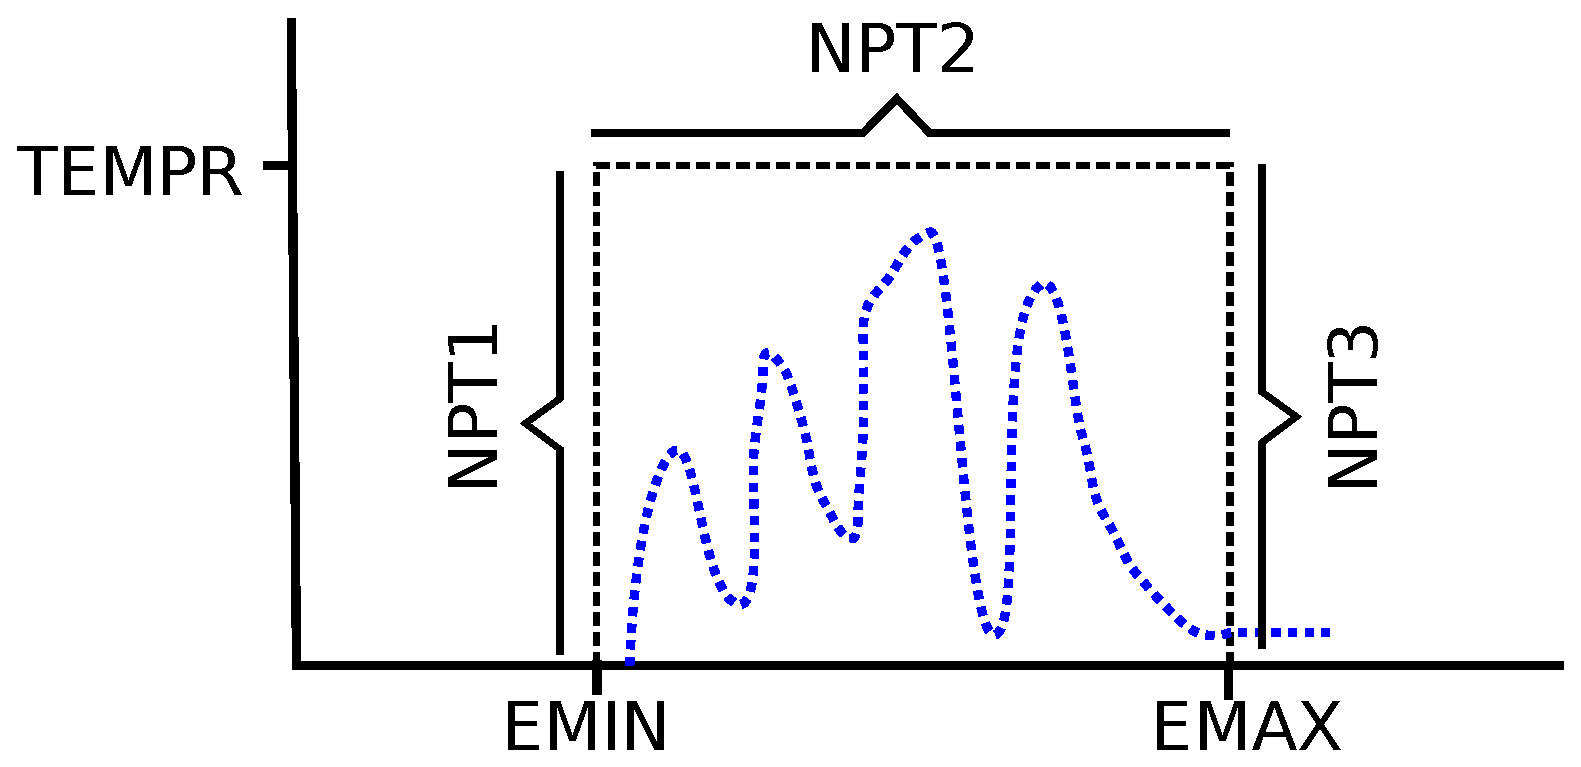
\includegraphics[width=\textwidth]{./EContour.eps}
\caption{Sketch of the energy contour as defined by the parameters given in the \texttt{inputcard}.\label{fig:EContour}}
\end{figure}


\begin{fBox}

{\Large{\textbf{\sffamily\textcolor{FZJTeal}{Tip: Check your electrons}}}}
To ensure a physically correct calculation one must check that the energy contour defined is such that all the valence electrons are actually included inside the defined area. This can be done by performing a one-shot calculation and checking that the number of electrons inside the contour is the appropiate for the studied system. This can be of great importance to describe systems that contain semicore states.

It is also critical to ensure that the Fermi energy is inside the Energy contour, a priori this is not known so the user must define a width of the contour large enough as to ensure that all the critical quantities are properly represented
\end{fBox} 

\subsection{Atomic info}\index{ATOMINFO}


%%%%%%%%%%%%%%%%%%%%%%%%%%%%%%%%%
%%%%%%%%%%%%%%%%%%%%%%%%%%%%%%%%%

\section{\texttt{VORONOI} program}\index{VORONOI}
\label{sec:voronoi}

To run the \verb;JM-KKR; program one first needs to create a series of files. One of the crucial files is the \textbf{\texttt{potential}} file, which as its name states will contain the information for the \textit{starting} guess of the potential for each one of the atoms in the unit cell. 

To create this file one needs the  

Before we run the KKR program, we need to create at least
the potential file (possibly more files too) using the VORONOI
program. This step requires of the \textbf{inputcard}, which should
be basically the inputcard to be used in the KKR calculation
for the new system. Then, take the time and write a proper
inputcard with all relevant parameters adjusted to the new system.
Copy it to the home directory of VORONOI.


We have to take special care of the 'I13' flag in the
inputcard, since this points to an already existing potential file.
There are two options (that I know so far):

\begin{itemize}
\item We dont have a previously generated potential file, i.e. we start from
scratch. Then, there should be no name in the line where the 'I13' flag appears
in the inputcard:
\begin{VBox}
\begin{verbatim}
FILES
4Ryshift                                      I12
                                              I13
\end{verbatim}
\end{VBox}

\item We have a potential file we want to use as a starting point for the
VORONOI program. Then, we need to copy it to the home directory of VORONOI,
and insert its name in the line where the 'I13' flag appears
in the inputcard. (This is the case, for instance, if we have generated the
\textbf{fort.3} potential file using a previous calculation.

\begin{VBox}
\begin{verbatim}
FILES
4Ryshift                                      I12
fort.3                                        I13
\end{verbatim}
\end{VBox}
)

\end{itemize}

Execute the program. The output potential is named 'output.pot', which must
be copied to the folder in which we will perform the KKR calculation.
Another possible output file of VORONOI is 'shapefun', used for full-potential
calculations (see Sec. \ref{sec:fp}).


Another important thing to check at this point is the number of atoms entering the scattering problem.
This is determined by the size of the TB cluster,
ie the RCLUSTZ and RCLUSTXY (see Sec. \ref{subsec:parameters}).
The important thing is that not \textit{too many} or \textit{too few} atoms enter: for \textit{normal}
calculations (bulk Si, Ag, Fe ...) around 60 atoms seems OK.
This can be checked \textbf{at the bottom of the output file}.

One has also to check the keyword 'clusters':
\begin{VBox}
{\small{
\begin{verbatim}
 CLSGEN_VORONOI: Atom            1  has cluster            1  with           55
  sites
 CLSGEN_VORONOI: Atom            2  has cluster            1  with           55
  sites
 CLSGEN_VORONOI: Atom            3  has cluster            1  with           55
  sites
 CLSGEN_VORONOI: Atom            4  has cluster            1  with           55
  sites
 CLSGEN_VORONOI: Atom            5  has cluster            1  with           55
...
\end{verbatim}
}}
\end{VBox}
If we have not entered the atomic positions or direct lattice with enough precission,
VORONOI may consider atoms that should in principle be equal (environment)
not equal. In the above, all atoms have been given the same cluster label.

\section{Running KKR program}
\label{sec:run-kkr}

Make a new directory for running the KKR program. There, the indispensable files
should be the inputcard, potential file and the executable file which
will run the different KKR executables (\textit{tbkkr\_run}).

First steps that must always be done:

\begin{itemize}
\item Think if we need to compile the KKR program or not. In any case, \textbf{remember
to set the right path-directory
for the KKR executables} in \textit{tbkkr\_run}.

\item Copy the potential file given by VORONOI
(default name 'output.pot') to current directory. Ideally,
name it 'potential', and insert this name in the line where the 'I13' flag appears
in the inputcard:
\begin{VBox}
\begin{verbatim}
FILES
4Ryshift                                      I12
potential                                     I13
\end{verbatim}
\end{VBox}
\end{itemize}


\subsection{Some parameters that are frequently changed}
\label{subsec:parameters}

\begin{itemize}

\item Number of atoms.

It is controlled by the parameters NAEZ and NTYPE, set them to be the number of atoms in the
unit cell. Sometimes it is desirable to insert 'empty' atoms to fill the otherwise empty
space between real atoms. The below describes two empty atoms introduced in bulk Si along
the unit cell diagonal at (0.5 0.5 0.5) and (0.75 0.75 0.75):
\begin{VBox}
{\small{
\begin{verbatim}
ATOMINFO
Z     LMXC    KFG     CLS   REFPOT   NTC    FAC    IRNS   RMT     WGHT
14.0   1      2 2 0 0    1      1       1     1.00    1   2.2d0   1.0d0
14.0   1      2 2 0 0    1      1       1     1.00    1   2.2d0   1.0d0
0.0    0      0 0 0 0    1      1       1     1.00    1   2.2d0   1.0d0
0.0    0      0 0 0 0    1      1       1     1.00    1   2.2d0   1.0d0
RBASIS
        0.00000    0.00000    0.00000
        0.25000    0.25000    0.25000
        0.50000    0.50000    0.50000
        0.75000    0.75000    0.75000
\end{verbatim}
}}
\end{VBox}

Thus, we set all 'zeros' in the empty atoms.

\item RCLUSTZ and RCLUSTXY.

This parameters, which are in units of the \textbf{lattice constant} (not Bohr),
determine the size of the TB cluster. Roughly, they determine the number of atoms
that will enter in the scattering problem (~). This should be checked
in the output of VORONOI
\end{itemize}

\subsection{SCF}

Here we list the parameters that somehow are related to the SCF calculation of the potential.

\begin{itemize}

\item Energy contour.

The parameters below are related to the (complex) energy integration contour:
\begin{VBox}
\begin{verbatim}
EMIN      EMAX       TEMPR      NPOL      NPT1    NPT2     NPT3
-0.30     0.9         502.57d0    5         3       20       2
\end{verbatim}
\end{VBox}
NPOL is number of Matsubara poles. NPT1,2,3 are number of energy points
to be calculated when going up in complex axis (at EMIN),
right in real axis (from EMIN to EMAX), and down in complex axis (at EMAX), respectively.



\item Number of iterations, potential mixing, convergence threshold (...)

The below parameters are characteristic of an SCF calculation:
\begin{VBox}
\begin{verbatim}
NSTEPS     IMIX    STRMIX       FCM       QBOUND    BRYMIX      ITDBRY
 100        4      0.050         20.0      1.D-8      0.06        40
\end{verbatim}
\end{VBox}

\begin{itemize}
\item NSTEPS, maximum number of SCF iterations, should be definitely bigger than 1.
\item QBOUND is the charge convergence threshold
\item STRMIX and BRYMIX control the percentage of the 'old' potential that is discarded
(i.e the potential of the previous iteration).
If we see that the charge is oscillating very much during the iterations, we may need to lower
the values of these parameters. This way, the program keeps a 'larger part' of the previous potential,
avoiding oscillations ($~$).
\end{itemize}




\end{itemize}

\subsection{DOS}

First of all, copy the selfconsistent potential to the folder in which we
will execute the KKR program for the DOS calculation.
Next, we insert some changes into the inputcard that we have used
for the SCF calculation.

\begin{itemize}

\item Insert keyword DOS:
\begin{VBox}
\begin{verbatim}
RUNOPT
full inv        DOS     ...
+-------+-------+-------+-------+-------+
\end{verbatim}
\end{VBox}

\item Set appropriate energy contour integration path, i.e points only
when moving along the real axis (NPT2):
\begin{VBox}
\begin{verbatim}
EMIN      EMAX       TEMPR      NPOL      NPT1    NPT2     NPT3
-0.20     0.9         502.57d0    0         0      110       0
\end{verbatim}
\end{VBox}
Note that we can change the temperature (TEMPR) for different DOS calculations.
This will change the 'smearing' used in the calculation of the delta functions
for the DOS; the smaller T, the smaller smearing, thus we usually need more
k-points for low T.

\item Set only one cycle in the inputcard, NSTEPS=1.

\end{itemize}


\subsection{Magnetic calculation}
\begin{itemize}

\item Compile the KKR program with parameter KSP = 1  in file inc.p.

\item KKR calculation. Start from a paramagnetic inputcard. Then, the following parameters have to be changed:

\begin{tabular}{ l | c | c |  c | c | c }
      & KHFELD\verb;*; & HFIELD & LINIPOL & INIPOL & NSPIN \\
  \hline
  Non-magnetic & 0 & 0.0 & f & 0 & 1 \\
  Magnetic  & 1 & finite value & t & 1 & 2 \\
\end{tabular}

(* Note how the variable 'KHFELD' is not written the same way as in the users guide 'KF{\kol I}ELD')
This will insert a magnetic field \textbf{only at the first SCF iteration}.
Then, if the starting potential was the minimum of the nonmagnetic case,
we need to apply a sufficiently strong magnetic field for the first iteration
so that it perturbs the potential enough to drive it away from the nonmagnetic
(local) minimum. This can be, for instance, 0.1 Ry in case of Iron.
We should look into the output.2 file to check if the system develops
a finite magnetic moment.

\item When having more than one magnetic atom in the unit cell, it is the
variable \verb|XINIPOL| that has to be used, not \verb|INIPOL|.
The program will expect to have as many integers after \verb|XINIPOL|
as different number of atoms we have, ie \verb|NATYP|. As an example,
if  \verb|NATYP=5|, then \verb|XINIPOL 1 0 0 1 0|, where the 1's and 0's
determine wether the magnetic field will be applied (1) or not (0)
to the corresponding atom (this we can choose).
This has not been tested by me, Prof. Ziane did it.

\end{itemize}

%%%%%%%%%%%%%%%
%%%%%%%%%%%%%%%
\section{Full Potential (FP)}
\label{sec:fp}

Here we describe the main steps

\begin{itemize}

\item If we want to use FP method, it is desirable to first run a calculation based on
the 'atomic sphere approximation' (ASA). We suppose here that
this is the case, i.e. that a succesfull SCF ASA calculation has been
performed in the system we want to study. Then, in the
SCF ASA inputcard, insert flag 'GENPOT' in the RUNOPT section:
\begin{VBox}
\begin{verbatim}
RUNOPT
full inv        GENPOT  ...
+-------+-------+-------+-------+-------+
\end{verbatim}
\end{VBox}

Run \textbf{kkr0.exe}, it should generate a file named
'fort.3', which has the right format to be read by VORONOI.

\item  VORONOI.

Copy the file 'fort.3' to the home directory of the VORONOI program.
At this step, we basically need the inputcard for the FP calculation.
For this, we need to change several flags compared to the ASA calculation.
These are:

\begin{tabular}{ l | c | c |  c | c | c}
      & IRNS & KSHAPE & IRM & INS & ICST \\
  \hline
  ASA & 1 & 0 & 349 & 0 & 2 \\
  FP  & 135 & 2 & 484 & 1 & 3 \\
\end{tabular}

Also, insert 'fort.3' name into the inputcard in the place marked
by I13:
\begin{VBox}
\begin{verbatim}
----------------------------------------------------------------------
FILES
4Ryshift                                      I12
fort.3                                        I13
madelung                                      I40
shapefun                                      I19
scoef                                         I25
\end{verbatim}
\end{VBox}

Once these flags have been changed in the inputcard,
run VORONOI using this inputcard. The program should output the potential
in file 'output.pot' and the shape functions in file 'shapefun'


\item Compile.

Some of the parameters above mentioned enter also in the inc.p file, so
it is very likely that we may need to compile again the program. The
parameters to be changed are:
\begin{tabular}{ l | c | c |  c }
      & KNOSPH & IRMD & IRNSD \\
  \hline
  ASA & 0 & 349 & 1 \\
  FP  & 1 & 484 & 208 \\
\end{tabular}

Compile the program with these parameters, save the executables and the inc.p file
in a separate folder.

\item Run KKR program

For running the KKR program in FP mode, we need to copy the
previously generated potential (output.pot) and shapefun files from VORONOI
home folder to the folder where we execute the program. Also,
remember to point to the right executables in the \textit{tbkkr\_run}
executable file.

\end{itemize}



%%%%%%%%%%%%%%%%%%%%%%%%%
%%%%%%%%%%%%%%%%%%%%%%%%%

\section{Band structure calculation}
\label{sec:bandstructure}

\begin{itemize}


\item To calculate with the program given by Long (zulapi.exe), we need to use the following
flags:
\begin{VBox}
\begin{verbatim}
RUNOPT
full invBAND-STR        ...
+-------+-------+-------+-------+-------+
\end{verbatim}
\end{VBox}

\item The k-space path is set as
\begin{VBox}
\begin{verbatim}
----------------------------------------------------------------------
 DIRECNO= 1
 DIRECDEF
  50
 0.0   0.0   0.0    0.0   0.0  0.0   < Gamma
 0.0   0.0   1.0    0.0   0.0  0.0   < H
\end{verbatim}
\end{VBox}

Use always DIRECNO = 1, which means that only one k-space line
is calculated, from $\Gamma$ to H in the above case.
Otherwise, if we insert more than one line, then plotting
gets a bit messy due to the output format.

\item Long said that the values of RCLUSTZ and RCLUSTXY
should be higher than in normal scf calculations so that
we take into account $\sim$ 250 neighbors.

\item Set temperature to \textbf{zero} and choose the number of energy points (in real axis)
and energy window:
\begin{VBox}
\begin{verbatim}
----------------------------------------------------------------------
EMIN      EMAX       TEMPR      NPOL      NPT1    NPT2     NPT3
-0.20     0.8         0.0         0         0      110       0
----------------------------------------------------------------------
\end{verbatim}
\end{VBox}
\item Add variables NSPO, NSPOH and NCL$\_$IMP to the inputcard:
\begin{VBox}
\begin{verbatim}
+-------+-------+-------+-------+-------+
  LMAX=3    NSPIN=1   NATYP=4 NSPO=1 NSPOH=1 NCL_IMP=1
\end{verbatim}
\end{VBox}

\item Compiling: as in the standard KKR program, one has to change the inc.p file
of the bandstructure program accordingly to the used inputcard.
First, make clean and \verb|rm *o|. Then compile.
Usual variables that need to be changed:
\begin{itemize}
\item NATYPD controls the number of atoms in the unit cell
\item NSPDD controls the SOC
\item INSD controls whether the calculation
is ASA or FP
\end{itemize}

\item \textbf{Output}: the first three numbers are the
coordinates of the k points in reciprocal-basis coordinates,
units of $2\pi/a$. Next the real and imaginary parts of the energy, and finally
a variable in which we are so far not interested.
The first line corresponds to the minimum energy, and last one
the maximum energy, ie increasing order.
\end{itemize}

%%%%%%%%%%%%%%%%%%%%%%%%%
%%%%%%%%%%%%%%%%%%%%%%%%%

\section{Slab calculation}
\label{sec:slab}

A slab calculation is meant to model a system in which periodicity is not
present along at least one spatial direction. We can think of a surface, for instance.
To model this, one must first prepare the position of the atoms that conform the surface,
and also of vacuum layers at both sides of the surface. An example containing
9 Ag layers and 6 vacuum layers is given below:
\begin{VBox}
\begin{verbatim}
CARTESIAN= t
RBASIS
0.00000000    0.00000000    0.00000000
0.50000000    0.28867513    0.81649658
1.00000000    0.57735027    1.63299316
1.50000000    0.86602540    2.44948974
2.00000000    1.15470054    3.26598632
2.50000000    1.44337567    4.08248290
3.00000000    1.73205081    4.89897949
3.50000000    2.02072594    5.71547607
4.00000000    2.30940108    6.53197265
4.50000000    2.59807621    7.34846923
5.00000000    2.88675135    8.16496581
5.50000000    3.17542648    8.98146239
6.00000000    3.46410162    9.79795897
6.50000000    3.75277675   10.61445555
7.00000000    4.04145188   11.43095213
----------------------------------------------------------------------
ATOMINFO
Z     LMXC    KFG     CLS   REFPOT   NTC    FAC    IRNS   RMT     WGHT
0.0    0    0 0 0 0    1      1       1     1.00    1   2.3d0   1.0d0
0.0    0    0 0 0 0    1      1       1     1.00    1   2.3d0   1.0d0
0.0    0    0 0 0 0    1      1       1     1.00    1   2.3d0   1.0d0
47.0   2    4 4 3 0    1      1       1     1.00    1   2.3d0   1.0d0
47.0   2    4 4 3 0    1      1       1     1.00    1   2.3d0   1.0d0
47.0   2    4 4 3 0    1      1       1     1.00    1   2.3d0   1.0d0
47.0   2    4 4 3 0    1      1       1     1.00    1   2.3d0   1.0d0
47.0   2    4 4 3 0    1      1       1     1.00    1   2.3d0   1.0d0
47.0   2    4 4 3 0    1      1       1     1.00    1   2.3d0   1.0d0
47.0   2    4 4 3 0    1      1       1     1.00    1   2.3d0   1.0d0
47.0   2    4 4 3 0    1      1       1     1.00    1   2.3d0   1.0d0
47.0   2    4 4 3 0    1      1       1     1.00    1   2.3d0   1.0d0
0.0    0    0 0 0 0    1      1       1     1.00    1   2.3d0   1.0d0
0.0    0    0 0 0 0    1      1       1     1.00    1   2.3d0   1.0d0
0.0    0    0 0 0 0    1      1       1     1.00    1   2.3d0   1.0d0
\end{verbatim}
\end{VBox}
Note that vacuum layers are located in both sides of the surface.
This is important since for the slab calculation
connects both sides to an 'infinite' vacuum (the system is not
periodic along this direction in the program). Then,
we need to specify the next vacuum layer in both
sides, as shown below.

\subsection{Parameters}

\begin{itemize}

\item INTERFACE: set to TRUE

\item Quit option 'full inv' from the top of the inputcard

\item Set third vector of the Bravais lattice to zero:

\begin{VBox}
\begin{verbatim}
BRAVAIS
  1.00000000 0.00000000   0.00000000
  0.50000000 0.86602540   0.00000000
  0.00000000 0.00000000   0.00000000
\end{verbatim}
\end{VBox}

\item LEFTBASIS, RIGHBASIS: contain the location of the 'next' vacuum layer
\begin{VBox}
\begin{verbatim}
LEFTBASIS    X         Y         Z     REFPOT
     -0.50000000  -0.28867513  -0.81649658  1  1
RIGHBASIS
      7.50000000   4.33012701  12.24744871  1  1
\end{verbatim}
\end{VBox}

\item NLEFTHOS, NRIGHTHO: number of times that the vacuum layer defined in
LEFTBASIS, RIGHBASIS will be repeated on top by the program

\item NLBASIS, NRBASIS: number of layers declared in LEFTBASIS, RIGHBASIS, ie 1

\item ZPERIODL, ZPERIODR: the real space direction in which the layers at
left/right will be repeated. This is usually given by the 2nd layer contained in RBASIS,
se the example below
\end{itemize}
Example:
\begin{VBox}
\begin{verbatim}
INTERFACE= T
NRIGHTHO=  12    NLBASIS=  1
NLEFTHOS=  12    NRBASIS=  1
LEFTBASIS    X         Y         Z     REFPOT
     -0.50000000  -0.28867513  -0.81649658  1  1
RIGHBASIS
      7.50000000   4.33012701  12.24744871  1  1
---------------------------------------
ZPERIODL= -0.50000000  -0.28867513  -0.81649658
ZPERIODR= 0.50000000  0.28867513  0.81649658
\end{verbatim}
\end{VBox}


\subsection{Things to check/tricks}
Before running the full KKR program, it is good to only run
kkr0 and check the output file output.0. There, look for the line
\begin{VBox}
\begin{verbatim}
********** TESTING THE COUPLING MATRIX ********
\end{verbatim}
\end{VBox}
Just below of it, the program says something about a variable called
NPRINCD. Still Im not sure how to properly set this value
(it has something to do with the blocks of the band diagonal matrix appearing
just above this point), but from Manuels
advices, one should not always trust the recommendation of the program at this point.
So far, using 15 layers (atoms + vacuum) we have used option NPRINCD=3.
I think that if we have had an even number of layers, then NPRINCD=2 would have been preferable.
This parameter has to be changed in inc.p file, and recompile the program.

\subsection{Non-symmetric positions, relaxed structure}

It is sometimes desirable to locate an impurity in a position
that does not follow the symmetry of the underlying structure.
This is usually done because we will eventually want to insert an impurity
in that position. We know that impurities tend to approach the surface,
so that its real (relaxed) distance along the surface perpendicular direction
can vary as much as $25\%$ as compared to the non-relaxed one. This can have an impact on
the electronic structure.

We have to go back to the Voronoi step for constructing the potential.
There, we use the new inputcard that contains the relaxed position of the impurity (on vacuum):
\begin{VBox}
\begin{verbatim}
RBASIS
0.00000000    0.00000000   0.00000000
0.50000000    0.50000000   0.70710678
0.00000000    0.00000000   1.52027957 <-- this was 1.41421356 in the relaxed case
0.50000000    0.50000000   2.12132034     now it contains a 15% relaxation with respect to the
0.00000000    0.00000000   2.82842712     surface layer
...
\end{verbatim}
\end{VBox}
Above, vacuum position just on top of the surface atom
has been reduced by 15$\%$, from 1.41421356 to 1.52027957
(the distance has been reduced with respect to 2.12132034, the position
of the surface layer).
Note that in this case we did not change the position of the rest
of vacuum sites.

We execute VORONOI with this new inputcard, and take a look to the output.
The main change is that now there are more different TB cluster types.
Check this part:
\begin{VBox}
\begin{verbatim}
Atom            1  has cluster            1
...
Atom            1  has cluster            2
...
Atom            6  has cluster            6
Atom            6  has cluster            6
Atom            6  has cluster            6
\end{verbatim}
\end{VBox}
Because of our modification of the position, the neighboring sites will have different TB
clusters. The ones that are very  far away from our modified position will have the
same cluster type. In the above example, 6 different clusters were found. This is an
important number, as it has to go into the \textbf{inc.cls} file for
the compilation of the JM program.

So we go now to the JM folder, and recompile, inserting the correct value in
the \textbf{inc.cls} file, setting the value of the parameter NCLSD to
the maximum number of different clusters outputed by VORONOI: NCLSD=6 in the case
studied above.

Now save and store the executables in a folder. For running the
program, first copy the output potential of VORONOI, output.pot,
to the folder where we will make the calculations. If we have a previously converged
potential for the symmetric position of the vacuum (no relaxation),
we can take advantage of it, and just copy the potential of the site that
we have modified into the converged potential (maybe the neighborinig sites too).
The last thing is to specify in the inputcard which type of cluster corresponds to
each atom, which as we have seen is declared in the output of the VORONOI program.
This is specified in the ATOMINFO part, parameter CLS:
\begin{VBox}
{\small{
\begin{verbatim}                      |||
ATOMINFO              vvv
Z     LMXC    KFG     CLS   REFPOT   NTC    FAC    IRNS   RMT     WGHT
0.0    0    0 0 0 0    1      1       1     1.00    1   2.3d0   1.0d0
0.0    0    0 0 0 0    2      1       1     1.00    1   2.3d0   1.0d0
0.0    0    0 0 0 0    3      1       1     1.00    1   2.3d0   1.0d0
47.0   2    4 4 3 0    4      1       1     1.00    1   2.3d0   1.0d0
47.0   2    4 4 3 0    5      1       1     1.00    1   2.3d0   1.0d0
47.0   2    4 4 3 0    6      1       1     1.00    1   2.3d0   1.0d0
47.0   2    4 4 3 0    6      1       1     1.00    1   2.3d0   1.0d0
47.0   2    4 4 3 0    6      1       1     1.00    1   2.3d0   1.0d0
47.0   2    4 4 3 0    6      1       1     1.00    1   2.3d0   1.0d0
47.0   2    4 4 3 0    6      1       1     1.00    1   2.3d0   1.0d0
47.0   2    4 4 3 0    6      1       1     1.00    1   2.3d0   1.0d0
47.0   2    4 4 3 0    6      1       1     1.00    1   2.3d0   1.0d0
47.0   2    4 4 3 0    6      1       1     1.00    1   2.3d0   1.0d0
47.0   2    4 4 3 0    6      1       1     1.00    1   2.3d0   1.0d0
47.0   2    4 4 3 0    6      1       1     1.00    1   2.3d0   1.0d0
0.0    0    0 0 0 0    6      1       1     1.00    1   2.3d0   1.0d0
0.0    0    0 0 0 0    6      1       1     1.00    1   2.3d0   1.0d0
0.0    0    0 0 0 0    6      1       1     1.00    1   2.3d0   1.0d0
\end{verbatim}
}}
\end{VBox}

%%%%%%%%%%%%%%%%%%%%%%%%%%%%%%%%%%%%%%
%%%%%%%%%%%%%%%%%%%%%%%%%%%%%%%%%%%%%%
\subsection{Version of JM code with only one executable}

In the currently (04/2016) newest version of the JM code only one executable is needed.
An important issue in this version is the variable \verb|WLENGTH| in inc.p
file. As far as I know, this has to do with the dimensions of the
\verb|kkrflex_*| files that are outputed for a impurity calculation (see next section).
From what I understand, for "old" versions of the impurity code (the ones that currently
have been connected to Manuels SOC solver) we need to set \verb|WLENGTH=4|,
while for the newest versions of the impurity code (that have to date not been connected to
Manuels SOC solver) we need to set  \verb|WLENGTH=1|. If we do not take care of this,
the calculation may crash at the stage of the impurity step.


%----------------------------------------------------------------------------------------
%	CHAPTER 3 KKRFFLEX
%----------------------------------------------------------------------------------------
\chapter{KKRFLEX}

\section{Impurity calculation}
\label{sec:impurity}

The first step for an impurity calculation is to decide where we will put the
impurity in real space. Typically, this can be in the first vacuum layer,
just on top of the last surface layer. Here we follow an example
of the Ag(100) surface; the starting point is the
inputcard for the Ag(100) slab.
Here we show the 3 vacuum layers and first
Ag surface layers taken from the slab inputcard
\begin{VBox}
{\small{
\begin{verbatim}
ATOMINFO
Z     LMXC    KFG     CLS   REFPOT   NTC    FAC    IRNS   RMT     WGHT
0.0    0      0 0 0 0    1      1       1     1.00    1   2.3d0   1.0d0
0.0    0      0 0 0 0    1      1       1     1.00    1   2.3d0   1.0d0
0.0    0      0 0 0 0    1      1       1     1.00    1   2.3d0   1.0d0  <-- we choose this one,
47.0   2      4 4 3 0    1      1       1     1.00    1   2.3d0   1.0d0      3rd place!
47.0   2      4 4 3 0    1      1       1     1.00    1   2.3d0   1.0d0
...
\end{verbatim}
}}
\end{VBox}
We have indicated the location in the vacuum where we will insert our impurity,
which is the one corresponding to the third position.
Then, we need to extract information regarding the neighbors of this site.
To do that, we have to run 1 cycle using the inputcard of the slab,
with the flag \textbf{clusters}:
\begin{VBox}
\begin{verbatim}
RUNOPT
clusters        ...     ...
+-------+-------+-------+-------+-------+
\end{verbatim} 
\end{VBox}

This will output a file called clusters. In there, we have information
regarding the neighbors of all sites defined in our slab:
\begin{VBox}
{\tiny{
\begin{verbatim}
  18 <--number of sites
   5.4590000      ALAT
# Z       0.  0.  0. 47. 47. 47. 47. 47. 47. 47. 47. 47. 47. 47. 47.  0.  0.  0.
# KAOEZ    1   2   3   4   5   6   7   8   9  10  11  12  13  14  15  16  17  18
      55 <-- number of neighbors of each site
       1       1  #---  information regarding the neighbors of the FIRST site (as defined in inputcard)
  0.0000000000000000000E+00  0.0000000000000000000E+00  0.0000000000000000000E+00    1  0.0  0.000000000E+00
 -0.5000000000000000000E+00 -0.5000000000000000000E+00 -0.7071067811865475727E+00  -19  0.0  0.100000000E+01
  0.5000000000000000000E+00 -0.5000000000000000000E+00 -0.7071067811865475727E+00  -19  0.0  0.100000000E+01
 -0.5000000000000000000E+00  0.5000000000000000000E+00 -0.7071067811865475727E+00  -19  0.0  0.100000000E+01
^
|
| Total of 55 neighbors
|
v
      55
       2       1  #---  information regarding the neighbors of the SECOND site
  0.0000000000000000000E+00  0.0000000000000000000E+00  0.0000000000000000000E+00    2  0.0  0.000000000E+00
^
|
| Total of 55 neighbors
|
v
      55
       3       1  #---  information regarding the neighbors of the THIRD site, the one we want!
  0.0000000000000000000E+00  0.0000000000000000000E+00  0.0000000000000000000E+00    3  0.0  0.000000000E+00
 -0.5000000000000000000E+00 -0.5000000000000000000E+00 -0.7071067811865475727E+00    2  0.0  0.100000000E+01
  0.5000000000000000000E+00 -0.5000000000000000000E+00 -0.7071067811865475727E+00    2  0.0  0.100000000E+01
 -0.5000000000000000000E+00  0.5000000000000000000E+00 -0.7071067811865475727E+00    2  0.0  0.100000000E+01
  0.5000000000000000000E+00  0.5000000000000000000E+00 -0.7071067811865475727E+00    2  0.0  0.100000000E+01
  0.0000000000000000000E+00 -0.1000000000000000000E+01  0.0000000000000000000E+00    3  0.0  0.100000000E+01
 -0.1000000000000000000E+01  0.0000000000000000000E+00  0.0000000000000000000E+00    3  0.0  0.100000000E+01
  0.1000000000000000000E+01  0.0000000000000000000E+00  0.0000000000000000000E+00    3  0.0  0.100000000E+01
  0.0000000000000000000E+00  0.1000000000000000000E+01  0.0000000000000000000E+00    3  0.0  0.100000000E+01
 -0.5000000000000000000E+00 -0.5000000000000000000E+00  0.7071067811865475727E+00    4 47.0  0.100000000E+01
  0.5000000000000000000E+00 -0.5000000000000000000E+00  0.7071067811865475727E+00    4 47.0  0.100000000E+01
 -0.5000000000000000000E+00  0.5000000000000000000E+00  0.7071067811865475727E+00    4 47.0  0.100000000E+01
  0.5000000000000000000E+00  0.5000000000000000000E+00  0.7071067811865475727E+00    4 47.0  0.100000000E+01
  0.0000000000000000000E+00  0.0000000000000000000E+00 -0.1414213562373095145E+01    1  0.0  0.141421356E+01
 -0.1000000000000000000E+01 -0.1000000000000000000E+01  0.0000000000000000000E+00    3  0.0  0.141421356E+01
  0.1000000000000000000E+01 -0.1000000000000000000E+01  0.0000000000000000000E+00    3  0.0  0.141421356E+01
 -0.1000000000000000000E+01  0.1000000000000000000E+01  0.0000000000000000000E+00    3  0.0  0.141421356E+01
  0.1000000000000000000E+01  0.1000000000000000000E+01  0.0000000000000000000E+00    3  0.0  0.141421356E+01
  0.0000000000000000000E+00  0.0000000000000000000E+00  0.1414213562373095145E+01    5 47.0  0.141421356E+01
  0.0000000000000000000E+00 -0.1000000000000000000E+01 -0.1414213562373095145E+01    1  0.0  0.173205081E+01
 -0.1000000000000000000E+01  0.0000000000000000000E+00 -0.1414213562373095145E+01    1  0.0  0.173205081E+01
  0.1000000000000000000E+01  0.0000000000000000000E+00 -0.1414213562373095145E+01    1  0.0  0.173205081E+01
^
|
| Total of 55 neighbors
|
v
...
\end{verbatim}
}}
\end{VBox}

Then, from the 3rd site, we need to choose the number of neighbors that we will take into account
for the impurity calculation.
We can check the distance from the origin in the last column.
In this example we could for example consider
the first 19 ones, up to distance 0.141421356E+01.
Then, we copy/paste these 19 lines from the 3rd site into a file called \textbf{scoef}
(first put the number of neighbors considered):
\begin{VBox}
{\tiny{
\begin{verbatim}
19
  0.0000000000000000000E+00  0.0000000000000000000E+00  0.0000000000000000000E+00    3  0.0  0.000000000E+00
 -0.5000000000000000000E+00 -0.5000000000000000000E+00 -0.7071067811865475727E+00    2  0.0  0.100000000E+01
  0.5000000000000000000E+00 -0.5000000000000000000E+00 -0.7071067811865475727E+00    2  0.0  0.100000000E+01
 -0.5000000000000000000E+00  0.5000000000000000000E+00 -0.7071067811865475727E+00    2  0.0  0.100000000E+01
  0.5000000000000000000E+00  0.5000000000000000000E+00 -0.7071067811865475727E+00    2  0.0  0.100000000E+01
  0.0000000000000000000E+00 -0.1000000000000000000E+01  0.0000000000000000000E+00    3  0.0  0.100000000E+01
 -0.1000000000000000000E+01  0.0000000000000000000E+00  0.0000000000000000000E+00    3  0.0  0.100000000E+01
  0.1000000000000000000E+01  0.0000000000000000000E+00  0.0000000000000000000E+00    3  0.0  0.100000000E+01
  0.0000000000000000000E+00  0.1000000000000000000E+01  0.0000000000000000000E+00    3  0.0  0.100000000E+01
 -0.5000000000000000000E+00 -0.5000000000000000000E+00  0.7071067811865475727E+00    4 47.0  0.100000000E+01
  0.5000000000000000000E+00 -0.5000000000000000000E+00  0.7071067811865475727E+00    4 47.0  0.100000000E+01
 -0.5000000000000000000E+00  0.5000000000000000000E+00  0.7071067811865475727E+00    4 47.0  0.100000000E+01
  0.5000000000000000000E+00  0.5000000000000000000E+00  0.7071067811865475727E+00    4 47.0  0.100000000E+01
  0.0000000000000000000E+00  0.0000000000000000000E+00 -0.1414213562373095145E+01    1  0.0  0.141421356E+01
 -0.1000000000000000000E+01 -0.1000000000000000000E+01  0.0000000000000000000E+00    3  0.0  0.141421356E+01
  0.1000000000000000000E+01 -0.1000000000000000000E+01  0.0000000000000000000E+00    3  0.0  0.141421356E+01
 -0.1000000000000000000E+01  0.1000000000000000000E+01  0.0000000000000000000E+00    3  0.0  0.141421356E+01
  0.1000000000000000000E+01  0.1000000000000000000E+01  0.0000000000000000000E+00    3  0.0  0.141421356E+01
  0.0000000000000000000E+00  0.0000000000000000000E+00  0.1414213562373095145E+01    5 47.0  0.141421356E+01
# put some empty lines and after the rest of the sites

  0.0000000000000000000E+00 -0.1000000000000000000E+01 -0.1414213562373095145E+01    1  0.0  0.173205081E+01
 -0.1000000000000000000E+01  0.0000000000000000000E+00 -0.1414213562373095145E+01    1  0.0  0.173205081E+01
 ...
\end{verbatim}
}}
\end{VBox}
We call the above the 'impurity cluster'.

Once we have created the scoef file,
we need to output some files that will be needed in the impurity calculation.
For this, copy the scoef file to a new folder together with the inputcard
and selfconsistent potential file of the Ag(100) slab.
Set these variables in the inputcard and the flag scoef:

\begin{VBox}
\begin{verbatim}
RUNOPT
KKRFLEX
...
IGREENFUN= 1        ICC= 1
...
KHFELD= 0
...
FILES
4Ryshift                                      I12
potential                                     I13
madelung                                      I40
shapefun                                      I19
scoef                                         I25
\end{verbatim}
\end{VBox}
Dont forget that the new version looks for \verb|KHFELD|, not \verb|KHFIELD|, scheize!!
Run \verb|tbkkr_run| (one iteration) with the recent version of the JM code by Philip
(the version by Phivos seems not to output what we need).
Use the executables compiled for the characteristics of the Ag100 slab.
The program should output these files:
\begin{VBox}
\begin{verbatim}
kkrflex_atominfo
kkrflex_green
kkrflex_hoststructure.dat
kkrflex_intercell_cmoms
kkrflex_intercell_ref
kkrflex_tmat
\end{verbatim}
\end{VBox}
%impurity.coefs
%intercell_ref
%green
which contain information needed in the impurity run.
Copy these files to another new directory where we will run the impurity program.


The final task before being able to run the impurity
program is to generate the \textbf{potential file corresponding to the
impurity cluster}.
We take a look back to the  scoef file (see above), and pay special attention to
the numbers in the 4th column; this tells us
the correspondence with the sites defined in the inputcard.
That is, in the example above, the first position in the impurity cluster
is equivalent to the third site defined in the inputcard. The next 4 lines are equivalent
to the second site defined in the inputcard, and so on.
In this example, we have up to 5 different sites in the impurity cluster. Then,
for generating the impurity potential file we start by opening the
selfconsistent potential of the slab, which contains information of
all the sites included in the inputcard, 18 in this example.
Then, we need to copy the potentials corresponding to the sites
of the impurity cluster, given by the numbers of the 4th column.
Unfortunately, \textbf{the name of the potential file
must be 'potential'}, as the kkrflex program looks
for a file named that way; we cannot therefore distinguish
by the name if it is a impurity potential file or a
'normal' one.
In this example, we need to copy the potentials corresponding to the
first 5 sites. We paste them into a new potential file
following the
order appearing in scoef: in this example, we need to insert in first place
the potential corresponding to the 3rd site. Then, insert the potential
corresponding to the 2nd site \textbf{4 times}. Then, insert the potential
corresponding to the 3rd site \textbf{4 times} also, and so on till we have inserted
as many potentials as sites in the impurity cluster, 19 in the present example.

\textbf{Use python script create-imp-pot.py}, it automatically creates the impurity potential,
it only needs the slab potential file and the scoef file, fancy!

\textit{Trick}: for copy/pasting the correct potentials, a nice way
is to write a label to the potentials we have to copy:
\begin{VBox}
\begin{verbatim}
Vac0 POTENTIAL  HOST 1              exc: Vosko,Wilk,Nusair
  2.30000000  5.45900000  2.29152538
   0.00000
   3.01702   0.590108635419487   0.913965251127118
...
Vac0 POTENTIAL   HOST 2             exc: Vosko,Wilk,Nusair
  2.30000000  5.45900000  2.29152538
   0.00000
   3.01702   0.590108635419487   0.913965251127118
349
...
Vac0 POTENTIAL    HOST 3            exc: Vosko,Wilk,Nusair
  2.30000000  5.45900000  2.29152538
   0.00000
   3.01702   0.590108635419487   0.913965251127118
349
...
Ag47 POTENTIAL   HOST 4             exc: Vosko,Wilk,Nusair
  2.30000000  5.45900000  2.29152538
  47.00000
   3.01702   0.590108635419487   0.913965251127118
...
Ag47 POTENTIAL    HOST 5            exc: Vosko,Wilk,Nusair
  2.30000000  5.45900000  2.29152538
  47.00000
   3.01702   0.590108635419487   0.913965251127118
349
...
\end{verbatim}
\end{VBox}
Then the copy/pasting is easier, and it will help to check whether the python
script worked well or not.

\subsection{Vacuum impurity}
\label{sec:vacuum-impurity}

Now we are in position to perform an impurity calculation. For this, we
first have to decide what atom-type will be the impurity. As a first test, we
will analyze what happens if we insert an 'vacuum impurity' atom.
For this, we dont need to change anything in the impurity potential file,
as originally there was vacuum in the position where we have chosen to insert the
impurity, and we have accordingly set a 'vacuum potential' in the first place.
Clearly, vacuum is not a real impurity, and should not therefore
affect the properties of the system.


We go to the directory where we have stored the output files mentioned above,
the impurity potential and inputcard. Also, we need to copy the file
\textbf{config.cfg}, there some variables for the calculation are defined.
We then execute the KKRFLEX\_source/SOURCE/\textbf{kkrflex.exe} program; this will try to find
convergence selfconsistently. If we have done the things properly, the system
should be near convergence starting from the first iterations, and should reach
convergence soon.

Once convergence is reached, the output is written to
file out\_log.000.txt, and the output potential
to out\_potential.
We can check the calculated charge density around each atom.
Type
\begin{VBox}
\begin{verbatim}
grep 'Atom' out_log.000.txt > impurity-charge.dat
\end{verbatim}
\end{VBox}
and check the charge in each atom in the last sclefconsistent cycle (at the bottom):
\begin{VBox}
\begin{verbatim}
  Atom    1 charge in wigner seitz sphere =    0.262375
  Atom    2 charge in wigner seitz sphere =    0.003933
  Atom    3 charge in wigner seitz sphere =    0.003933
  Atom    4 charge in wigner seitz sphere =    0.003933
  Atom    5 charge in wigner seitz sphere =    0.003933
  Atom    6 charge in wigner seitz sphere =    0.262375
  Atom    7 charge in wigner seitz sphere =    0.262375
  Atom    8 charge in wigner seitz sphere =    0.262375
  Atom    9 charge in wigner seitz sphere =    0.262375
  Atom   10 charge in wigner seitz sphere =   46.742070
  Atom   11 charge in wigner seitz sphere =   46.742070
  Atom   12 charge in wigner seitz sphere =   46.742070
  Atom   13 charge in wigner seitz sphere =   46.742070
  Atom   14 charge in wigner seitz sphere =    0.000029
  Atom   15 charge in wigner seitz sphere =    0.262375
  Atom   16 charge in wigner seitz sphere =    0.262375
  Atom   17 charge in wigner seitz sphere =    0.262375
  Atom   18 charge in wigner seitz sphere =    0.262375
  Atom   19 charge in wigner seitz sphere =   46.991713
\end{verbatim}
\end{VBox}
This has to be compared with the charge previously calculated in the scf run for the slab:
\begin{VBox}
\begin{verbatim}
grep 'Atom' output.2 > scf-charge.dat
\end{verbatim}
\end{VBox}
that gives:
\begin{VBox}
\begin{verbatim}
  Atom    1 charge in wigner seitz sphere =  0.000029
  Atom    2 charge in wigner seitz sphere =  0.003933
  Atom    3 charge in wigner seitz sphere =  0.262375
  Atom    4 charge in wigner seitz sphere = 46.742070
  Atom    5 charge in wigner seitz sphere = 46.991713
  Atom    6 charge in wigner seitz sphere = 46.999563
  Atom    7 charge in wigner seitz sphere = 46.999912
  Atom    8 charge in wigner seitz sphere = 47.000531
  Atom    9 charge in wigner seitz sphere = 46.999875
  Atom   10 charge in wigner seitz sphere = 46.999875
  Atom   11 charge in wigner seitz sphere = 47.000531
  Atom   12 charge in wigner seitz sphere = 46.999912
  Atom   13 charge in wigner seitz sphere = 46.999563
  Atom   14 charge in wigner seitz sphere = 46.991713
  Atom   15 charge in wigner seitz sphere = 46.742070
  Atom   16 charge in wigner seitz sphere =  0.262375
  Atom   17 charge in wigner seitz sphere =  0.003933
  Atom   18 charge in wigner seitz sphere =  0.000029
\end{verbatim}
\end{VBox}
We can see that the first charge in impurity-charge.dat
coincides with the third one of scf-charge.dat. In fact
we can find any of the 5 different charge values present in
impurity-charge.dat also in file scf-charge.dat, consistently with
how we have created the impurity cluster.

\subsection{Real impurity}
\label{sec:real-impurity}

Now we analyze how to introduce a 'real' impurity,
that is, a real atom in top of the surface.
We take as an example a Fe atom (nonmagnetic case).
First, we need to accordingly change the impurity potential file,
ie insert a Fe atom in place of the vacuum in the third site.
To do so, we copy the slab input card to VORONOI, and in place
of the vacuum, we insert the Iron atom:
\begin{VBox}
\begin{verbatim}
----------------------------------------------------------------------
ATOMINFO
Z     LMXC    KFG     CLS   REFPOT   NTC    FAC    IRNS   RMT     WGHT
0.0    0    0 0 0 0    1      1       1     1.00    1   2.3d0   1.0d0
0.0    0    0 0 0 0    1      1       1     1.00    1   2.3d0   1.0d0
26.0   1    3 3 0 0    1      1       1     1.00    1   2.3d0   1.0d0
47.0   2    4 4 3 0    1      1       1     1.00    1   2.3d0   1.0d0
47.0   2    4 4 3 0    1      1       1     1.00    1   2.3d0   1.0d0
...
\end{verbatim}
\end{VBox}
\textbf{Very important}: we need to use the same RMT radious
as for the vacuum in order to avoid incompatibilities.
VORONOI will output a potential with Fe in the third site.
From this potential file, copy the part corresponding to Fe:
\begin{VBox}
\begin{verbatim}
Fe26 POTENTIAL  HOST Fe             exc: von Barth,Hedin
  2.30000000  5.45900000  2.34954834
  26.00000
   3.01702   0.4092410000   0.5000000000
...
\end{verbatim}
\end{VBox}
and replace with it the first
vacuum potential of impurity-potential; namely,
erase the \textbf{first} vacuum potential and insert in its
place the Fe potential.
This will be our starting potential for the impurity run
in the 'real' case. Next, copy all the files needed by the impurity program
(the kkr\_ files and so on, also the config.cfg input file) to the present directory.
Before running the program, we need to change the
\textbf{atomic number} of the first place (now an Iron atom)
in file kkrflex\_atominfo:
\begin{VBox}
{\scriptsize{
\begin{verbatim}
0.0000000000000000       0.0000000000000000       0.0000000000000000 26.00       0      0     3
...
\end{verbatim}
}}
\end{VBox}
Now we can run the impurity program.
\subsection{Magnetic impurities}

Now we see how to include magnetism into the impurity calculation.
First of all, we need to double the number of potentials of the nonmagnetic potential file in order
to take into account the spin-up spin-down states.
The easiest way is to simply copy paste every nonmagnetic potential,
ie we set same (starting) potential for both spin directions. In the present example, we
would have $2\cdot19=38$ potentials:
\begin{VBox}
\begin{verbatim}
Fe26 POTENTIAL  HOST Fe             exc: Vosko,Wilk,Nusair
  2.30000000  5.45900000  2.30000000
  26.00000
   3.01702   0.5901086354   0.9139652511
349
 0.25000000D-01 0.50267689D-03
 5 1
    0  -5.12038694958D+02
    0  -5.88813480612D+01
...
\end{verbatim}
\end{VBox}

\noindent we copy the first nonmagnetic potential (belonging to the magnetic impurity Fe) and paste it just below
\begin{VBox}
\begin{verbatim}
Fe26 POTENTIAL  HOST Fe             exc: Vosko,Wilk,Nusair
  2.30000000  5.45900000  2.30000000
  26.00000
   3.01702   0.5901086354   0.9139652511
349
 0.25000000D-01 0.50267689D-03
 5 1
    0  -5.12038694958D+02
    0  -5.88813480612D+01
...
Vac0 POTENTIAL   HOST 2             exc: Vosko,Wilk,Nusair
  2.30000000  5.45900000  2.30000000
   0.00000
   3.01702   0.5901086354   0.9139652511
349
...
\end{verbatim}
\end{VBox}
\noindent copy the second nonmanetic potential and paste it below, and so on
\begin{VBox}
\begin{verbatim}
Vac0 POTENTIAL   HOST 2             exc: Vosko,Wilk,Nusair
  2.30000000  5.45900000  2.30000000
   0.00000
   3.01702   0.5901086354   0.9139652511
349
...
\end{verbatim}
\end{VBox}
The python script of David does quickly the job, run
\begin{VBox}
\begin{verbatim}
python modifypotential.py
\end{verbatim}
\end{VBox}
in a folder containing the nonmagnetic potential file 'potential', and choose the
input option 13. It will create the doubled potential 'new\_potential' that we can use
in a magnetic calculation.

Now we have to tell the program that we want to perform a spin-polarized magnetic calculation.
This is done via the inputcard of the impurity program, namely the
\textbf{config.cfg} file.
There we need to change the following parameters:
\begin{itemize}
\item NSPIN: this variable determines if a calculation will be magnetic or not:
\begin{VBox}
\begin{verbatim}
NSPIN= 2
# magnetic calculation
# NSPIN=1 non magnetic
# NSPIN=2 collinear magnetic calculation
\end{verbatim}
\end{VBox}
We set it to 2.

 \item HFIELD: this variable is used to apply a magnetic field in order to break the
symmetry of the nonmagnetic calculation; otherwise the system will converge to a nonmagnetic
minimum even if we perform a magnetic calculation and we know beforehand that the ground state
is magnetic. The magnetic field is introduced as
\begin{VBox}
\begin{verbatim}
 #       value(Ry)    how many iterations
HFIELD=   1.E-2              1
\end{verbatim}
\end{VBox}
The first value is the magnitude of the B field (in Rydberg), very big in the above example.
The second integer number is the number of iterations in which the magnetic field is applied.
One way of magnetizing our system is to apply a very strong field in the first iteration
in order to strongly break the nonmagnetic symmetry. Then, the program may (should)
be able to converge to a magnetic solution.

\textbf{Units} Note that if we want to apply a magnetic field of 1 Tesla, then we
have to introduce a magnetic field of $5.7883817555\cdot10^{-5}/13.6d0$.

\item IMIX. From experience of the KKR users, one usually needs to set \textbf{IMIX=0} (straight mixing)
in order to converge to a magnetic solution, at least in the first iterations, untill the program
starts to tend to a magnetic solution; then one can set \textbf{IMIX=4} (Broyden mixing),
which is generally faster.

\end{itemize}

\subsection{Impurity DOS}

To calculate the DOS with the impurity program (once convergence has been reached),
one has to add the flag 'ldos' to the RUNFLAG option
\begin{VBox}
\begin{verbatim}
#########################################
RUNFLAG= noforce_fullgmat ldos
#########################################
\end{verbatim}
\end{VBox}
and set only one iteration (make sure to use the converged potential).
This will generate a bunch of files containing the DOS
at every atom. If the calculation was magnetic, we find two
files per atom (spin up/down).

Where is, however, the information regarding the integration path, number of k-points,
or the temperature? All these quantities are meaningful for a DOS calculation,
but do not appear in the config.cfg input file. All this sort of information
is stored into the \textbf{kkr\_green} and \textbf{kkr\_tmat} files.
The ones we have used for the scf loop of the impurity contain the setup for a
scf calculation. Then, if we do a DOS impurity calculation using these files, we
will get the energies along a path proper for a scf calculation, namely including points along
the imaginary axis. Also the temperature is higher than in normal DOS calculations.
Therefore, we would essentially not get good results.

To set the proper quantities for a DOS calculation, we need to go back to the
step of generating the kkr\_ files with the kkr program.
That is, copy the scf potential (of the slab), the scoef file and the inputcard
we used to generate the kkr\_ files to a new folder (this has flag KKRFLEX in RUNOPT).
Open the inputcard and change the variables pertinent for a DOS calculation:
energy integration contour, temperature and k-points. Run
one iteration with the program by Phillip, which will output
new kkr\_ files. Copy the \textbf{kkr\_green} and \textbf{kkr\_tmat} files
to the folder in which we will perform the DOS impurity calculation.
There we have to copy also all the files previously calculated in the scf
run for the impurity, \textbf{except} the old files \textbf{kkr\_green} and \textbf{kkr\_tmat}
corresponding to the scf calculation.

\subsection{More than one impurity}

Inserting more than one impurity is essentially not different to
just one impurity. In particular, the DFT calculation using the JM will be the same,
since we do not define any impurity there.
The only difference is when building the impurity cluster.
Now, instead of inserting only one real atom in one of the vacuum positions,
we insert more than one. Then, usually we would like to have similar neighboring clusters
around each of the impurities. Note that some of the nearest neighbors of
these impurities are the same. If we would just copy/paste the neighoring positions
of each of the impurities from the clusters file, we would be counting some of the
positions twice, and this will crash the program.
Instead, we need to use a little program by Manuel.

Needed files are:
\begin{VBox}
\begin{verbatim}
inputcard  test_scoef scoef_maker
\end{verbatim}
\end{VBox}
where \verb|inputcard| is the inputcard of JM code, \verb|scoef_maker| is the
executable of the program and \verb|test_scoef| is the inputfile:

\begin{VBox}
\begin{verbatim}
# BRAVAIS: how many, alat, then (x,y,z)
  2  4.830  <-- lattice constant, take from JM inputcard
  1.000000  0.000000  0.000000  <-- a1 and a2, copy from JM inputcard
  0.500000  0.866025  0.000000
# RBASIS: how many, cartesian, then (x,y,z), then atomic number
  18  T  <-- how many atoms in inputcard, and if positions are given in cartesian or not
0.0  0.00000000  0.00000000 0.0  <-- positions of atoms, copy from JM inputcard
0.5  0.28867513  0.81649658 0.0
1.0  0.57735026  1.76948974 0.0
1.5  0.86602539  2.44948974 78.0
2.0  1.15470052  3.26598632 78.0
2.5  1.44337565  4.08248290 78.0
3.0  1.73205078  4.89897948 78.0
3.5  2.02072591  5.71547606 78.0
4.0  2.30940104  6.53197264 78.0
4.5  2.59807617  7.34846922 78.0
5.0  2.88675130  8.16496580 78.0
5.5  3.17542643  8.98146238 78.0
6.0  3.46410156  9.79795896 78.0
6.5  3.75277669 10.61445554 78.0
7.0  4.04145182 11.43095212 78.0
7.5  4.33012695 12.24744870 0.0
8.0  4.61880208 13.06394528 0.0
8.5  4.90747721 13.88044186 0.0
# RIMP: how many, max number of cluster atoms, then lattice coordinates, rcut, which rbasis
  3  10000 <-- first number: how many impurities we want, next number dont touch
  0  0  1.50  3 <-- first two numbers: coefficients of a1 and a2 pointing to the first impuirity.
  1  0  1.50  3     second number; distance that determines the number of neighboring atoms included
  0  1  1.50  3     into the impurity cluster
\end{verbatim}
\end{VBox}

\subsection{Irregular geometries}
For irregular geometries where the principal layer number is not very well defined,
we need to make use of the newest verion of the JM code. Few points to consider
\begin{itemize}
\item Ewald sum

Use the \textbf{newest version} which has implemented the 3d sum

Otherwise it is very tricky to converge if we use the 2D sum: one has to increase the \verb|GMAX|
and \verb|RMAX| parameters a lot, and the kkr0 step takes a few hours.

\item Converge \verb|NSHELD| parameter in \verb|inc.p| file

If we have many sites that are coupled we will need to increase by a lot the parameter
\verb|NSHELD|, to values $\sim 30000$

\item Converge \verb|NSHELL0| integer in \verb|ALL_SOURCE_FILES/shellgen2k.f| file

\textbf{Important}: \verb|NSHELL0| must be larger than \verb|NSHELD|, so we may have to
modify by hand this parameter inside the code (default value is 10000)



\item Memory:
\begin{itemize}
\item the compilation can break down if some arrays run out of memory, we need to
modify the line containing the flagsin the \verb|makefile| file:
\begin{VBox}
\begin{verbatim}
FFLAGS       =   -r8 -traceback -module  $(OBJ)
\end{verbatim}
\end{VBox}
add the flag \verb|-mcmodel=large|:
\begin{VBox}
\begin{verbatim}
FFLAGS       =  -mcmodel=large -r8 -traceback -module  $(OBJ)
\end{verbatim}
\end{VBox}
\textbf{important}: for some reason I now dont remember we need to compile in the \verb|iff260|
cluster, otherwise the \verb|-mcmodel=large | is not recognized, something to do with the version of
the compiler installed, always use the latest machine!

\item when running, arrays may also run out of memory at the allocation time. For instance,
the integers \verb|ISH| and \verb|JSH| can run out of memory in main1b.f. To try to avoid it,
run in the \verb|iff597| cluster - it has 64 Gb in each node - and serially but taking the full node
(ie ask for 16 CPU's but run serially).

\end{itemize}

\end{itemize}


\subsubsection{old fashioned: gofrin}

There is
a patch provided by Manuel and Flaviano called godfrin. For that we need a OLD version of the JM
code that incorporates this patch. Then, insert the keyword \verb|godfrin| into the \verb|RUNOPT|
in the inputcard for the JM code, and run the kkr0.exe executable. This should output
a file called \verb|couplings.dat|. Then, copy this file to a separate folder and run there
a little program called  \verb|block_partitioning.exe|. The output on the pipe out (dump it for instance to
\verb|out_block_part|) looks something like:
\begin{VBox}
\begin{verbatim}
bandwidth: min, max, avg, dev=      27      62      48      12
minsize, maxblock=      19       6
nblocks,imax=       2      12              12
minsum2, nblocks, blocksizes=    8357       2      31      86
nblocks,imax=       3      12             144
minsum2, nblocks, blocksizes=    5049       3      30      30      57
nblocks,imax=       4      12            1728
minsum2, nblocks, blocksizes=    3429       4      27      30      30      30
nblocks,imax=       5      12           20736
minsum2, nblocks, blocksizes=    3429       4      27      30      30      30
nblocks,imax=       6       3             243
minsum2, nblocks, blocksizes=    3429       4      27      30      30      30
\end{verbatim}
\end{VBox}
The interesting part is the last row. In this particular case it tells us that he finds 4 blocks
(2nd number in last row), of sizes 27, 30, 30 and 30. So what we have to do is to copy these last numbers
into a file called \verb|godfrin.dat|, that looks like this in this example:
\begin{VBox}
\begin{verbatim}
# na, nb, ldiag, lper, lpardiso; then bdims(1:nb)
 117  4  T  F  F
 27      30      30      30
\end{verbatim}
\end{VBox}
That is, in the first line we have
inserted the number of atomic sites defined in the inputcard (117, this you know from
JM inputcard), and the number of blocks (4), while in the second line we have inserted
the size of the blocks also given in the last line of \verb|out_block_part|.

Finally, copy the \verb|godfrin.dat| file to a folder and execute there the JM code
with the patch, this should be able to run scf runs even in irregular geometries.
IMPORTANT: copy the \verb|godfrin.dat| to the SYSTEM folders, ie modify \verb|tbkkr_run| file.

%----------------------------------------------------------------------------------------
%	CHAPTER 4 KKRSUSC
%----------------------------------------------------------------------------------------
\chapter{Calculating the susceptibility}
\label{ch:susc}


\section{KKRSUSC}
\label{sec:kkrsusc}

\subsection{Basic information}
\label{sec:kkrsusc-basic-info}

The KKRSUSC program is inserted \textbf{into the KKRFLEX program},
meaning that it doesnt have a own executable, the executable keeps
being \textbf{kkrflex.exe}.
This program currently does \textbf{not} compute the susceptibility, but
it outputs the necessary files to do so by a subsequent postprocessing program.
There are 2 types of files that come into play:
\begin{itemize}
\item Files that already exist in the original KKRFLEX  program.

These are  \verb|calctmat.f90|, \verb|energyloop.F90|, \verb|calctmatfull.f90|
and \verb|kkrflex.F90|. These files have been modified from the original
version in order to include the stuff of the susceptibility.
We have inserted the parts corresponding to the KKRSUSC program into the files corresponding
to the latest version of the KKRFLEX program (before it was implemented into an older version).
One should check compatibility, make tests etc.

\item Files that do not exist in the original KKRFLEX program.

These are
\verb|kkrsusc_prepare.f90| \verb|projection.F90| and  \verb|type_inpsusc.f90|.
The subroutines contained in these files are called by the files in the previous
point, but these ones do not alter or modify any of the arrays used by KKRFLEX,
they only compute and output new quantities, to be further processed.
In order to include these files into the structure, the \textbf{makefile}
has to include them when compiling together with the rest of the KKRFLEX program.
These files must be copied into the SOURCE  folder.




\end{itemize}

\subsection{Runflag in impurity inputcard}



To run the KKRSUSC program, first of all we need to insert the \textbf{runflag} \verb|kkrsusc|
into the \textbf{config.cfg} inputcard of the impurity program:
\begin{VBox}
\begin{verbatim}
#########################################
RUNFLAG= noforce_fullgmat  kkrsusc
#########################################
\end{verbatim}
\end{VBox}
This will tell the \textbf{kkrflex.exe} program that the user wants to make use of the
KKRSUSC options.


\subsection{Proper energy mesh}
\label{subsec:emeshdat}


Before going on with inputcards and executables, it is worth to
note that for calculating the susceptibility,
it will be desirable to calculate
the Green function and T-matrix in
energy points that are different from those used in the scf
calculation (of both the JM and KKRFLEX program).
The energies we would like to consider are
difficult to set up in
the JM inputcard.
The following steps have to be performed
to set up the energies we want:

\begin{itemize}

\item Create the energy mesh file emesh.dat.

For this purpose, there is a little
fortran code named emesh.f90 that does the job.
It is located in a separate folder, usually called \verb|create_emeshdat|,
look for it on the codes folder. Now we need to prepare a simple input card
(lets call it inputfile):
\begin{VBox}
\begin{verbatim}
5       # npanels
-0.4    0.1      1.3    0.1     11      0       # e1r e1i e2r e2i npts imesh (1 for cheby)
-0.4    0.075    1.3    0.075   21      0       # e1r e1i e2r e2i npts imesh (1 for cheby)
-0.4    0.05     1.3    0.05    31      0       # e1r e1i e2r e2i npts imesh (1 for cheby)
-0.4    0.025    1.3    0.025   41      0       # e1r e1i e2r e2i npts imesh (1 for cheby)
-0.4    0.010    1.3    0.010   51      0       # e1r e1i e2r e2i npts imesh (1 for cheby)
\end{verbatim}
\end{VBox}
The above defines 5 lines that are parallel to the real axis, that range from
-0.4 to 1.3 Ry, at imaginary energies 0.1,  0.075, 0.05, 0.025 and 0.010,
using 11, 21, 31, 41 and 51 energy points respectively. The program is executed as
\begin{VBox}
\begin{verbatim}
emesh < inputfile
\end{verbatim}
\end{VBox}
This will generate the important file \textbf{emesh.dat}, which contains all the energies
in the proper format.

\item (Re)Calculate the Green function and T matrix using the JM code.

Now we have to perform a new calculation with the JM code to calculate
all the stuff in the energy points contained in emesh.dat.
First, copy the just created emesh.dat file to the directory where calculations will
be performed. Copy also the \textbf{inputcard and converged potential} files
that were used to compute the slab calculation using the JM code.
Finally, copy also the \textbf{scoef} file with the appropriate
information regarding the impurity cluster.
Next, we need to tell the JM code that we want to use the file emesh.dat for
the energies (not the path defined in the inputcard).
For this, in the fortran file \verb|SRC_COM_QDOS/main0.f| of the JM code
there is a few extra lines (search for \verb|!susc|).
Then, when we add the runflag KKRSUSC to \textbf{the inputcard of the JM code}
(inputcard):
\begin{VBox}
\begin{verbatim}
***** Input file for TB-KKR code *****
      ***Running options***
RUNOPT
KKRFLEX KKRSUSC ...     ...
+-------+-------+-------+-------+-------+
\end{verbatim}
\end{VBox}
The program will look for a emesh.dat file in the directory.
Note that in order to be able to use the usual \verb|tbkkr_run|
script, we need to introduce a extra line so that it copies the emesh.dat
file from the directory where \verb|tbkkr_run| is executed to the \verb|SYSTEM|
folder. This should be:
\begin{VBox}
\begin{verbatim}
#=======================================================================
cp  $here/$input $local/$work_name/inputcard
#  JULEN
cp  $here/emesh.dat $local/$work_name/emesh.dat  # <-- extra line!
cp  $here/scoef $local/$work_name/scoef
\end{verbatim}
\end{VBox}
Then, \verb|qsub| the script. If everything goes well,
the program will run a single scf step and ouput all the quantities
calculated in the new energy mesh. Then, we need to copy the
\verb|kkrflex_green| and \verb|kkrflex_tmat| files to the
directory where we will perform the KKRSUSC calculations.

\textbf{Note 1}: the emesh.dat file is only needed at this step, and it is only
the JM program who needs it. Once the \verb|kkrflex_green| and \verb|kkrflex_tmat| files
have been calculated, they already contain the information on the new energy mesh.
This means that when we will execute the SELFE  program, even though we want to
use the energy mesh defined in emesh.dat, we dont actually need this file,
since its information is already in the two files mentioned above; the program
will then automatically detect that the energy mesh in these files does not coincide
with the energy mesh of the scf run (which in this case must be given in a separate
file, see below), and proceed consequently, without the need of emesh.dat.

\textbf{Note 2}: sometimes putting too many panels into emesh.dat can give error messages
in output.0 like:
\begin{VBox}
\begin{verbatim}
     Dimension ERROR: Please increase MAXMSHD to 12
                      in the programs < main0 > and < main1b >

\end{verbatim}
\end{VBox}
The source of this error is on how the k-mesh is re-structured by
the program for different imaginary parts of the energy. It can be found in
\verb|SRC_COM_QDOS/bzkmesh.f|. To avoid this, use
\verb|fix mesh| flag in the TESTOPT part of the JM inputcard:
\begin{VBox}
\begin{verbatim}
TESTOPT
ie      RMESH   clusters
verb0   fix mesh  !<-- this is the flag!
\end{verbatim}
\end{VBox}
This will disable the re-structuring routine, and we should not get the problem anymore.

\end{itemize}

\subsection{Proper inputcard, inpsusc.dat}

Now we see what is the specific inputcard that
the KKRSUSC program needs,
which we name \textbf{inpsusc.dat}.
It should look like something like this:
\begin{VBox}
\begin{verbatim}
 Data for dynamical susceptibility calculation
 ne, na, nbmax, nlmax, sra=
 30    1     1     2     0
 ngroup, igroup(1:ngroup)=
   1
   1  3  6  3
 Nb adatom
   1
 nspin, iwsusc(0:lmax), ewsusc(1:nbmax,0:lmax)
 2     1     0     1     0
   1     0.5901    0.010
   1     0.5901    0.010
\end{verbatim}
\end{VBox}
The variables are as follows:
\begin{itemize}

\item ne: number of energy points in which the Green function was calculated by
the JM code, ie the energy points present in the file \verb|inputcard|.
In case we have made use of the emesh.dat (see below), then the number of energy points
should match with the ones in this file.

\item na: number of atoms for which we compute the susceptibility and projected basis set.
In the case of an impurity, if we are only interested in what happens at the impurity
itself, then we would choose na=1.

\item nbmax: Maximum number of wavefunctions that will be used to project the basis in
any of the amgular momentum channels. That is, we can choose for instance to project
the 's' channel into 1 wavefunction, but we may want to use 2 wavefunctions for
the 'p' channel (for whatever reason). Then nbmax would have to be equal to 2.

\item nlmax: channel with maximum angular momentum that we consider.
If we consider only 's' channel, then this is equal to 0. If we consider only 'p'
channel, then this is equal to 1. If we consider 's' \textbf{and} 'p' channel, then this is also
equal to 1 (the disctintion between which channels to consider is done below, this
only sets the maximum).

\item sra=0

\item ngroup: number of groups in which we will divide the \textbf{atoms} we have considered.
$ngroup>1$ could only be in the case that $na>1$.  The numbers below \verb|ngroup|
set the number of atoms in each group. In the example above, there is more
than one number in the line below \verb|ngroup|
even though na=ngroup=1; it doesnt matter, the program will only read the first number
as we have said that there is only one group, and ignore the rest.


\end{itemize}

Numbers inside the groups:

\begin{itemize}
\item

\begin{VBox}
\begin{verbatim}
 Nb adatom
   1
\end{verbatim}
\end{VBox}
This is very important, as here we specify which atom we are interested in.
Simplest example, na=ngroup=1. Even now, the program needs to know
which atom among all the atoms
present in the \textbf{impurity cluster} we are interested in. The label of each atom
is as in the \verb|potential| file or in the \verb|kkrflex_atominfo|,
ie usually atom number 1 is the impurity (as in this example),
next ones are some vacuums and so on.

\item
\begin{VBox}
\begin{verbatim}
 nspin,   iwsusc(0:lmax), ewsusc(1:nbmax,0:lmax)
 2     !(s) 1    !(p) 0   !(d) 1     0
   1     0.5901    0.010
   1     0.5901    0.010
\end{verbatim}
\end{VBox}
Put nspin = 2 always. Important thing is taht here we choose
the \textbf{angular momentum channels} to be considered.
This has to do with the variable lmaxd which we have defined previously.
Consider the case lmaxd=2. This means that we want to include at least the 'd'
channel, but what about the 's' and 'p'? We can choose to include or not all
this channels by setting 1 for yes or 0 for not 0 after declaring nspin.
In the example above, the 's' and 'd' channels are considered
but not the 'p' channel.  Then, accordingly we need to insert
2 lines below corresponding to the 2 channels considered.
\begin{VBox}
\begin{verbatim}
   1     0.5901    0.010
   1     0.5901    0.010
\end{verbatim}
\end{VBox}
In these lines, we first insert the label that identifies the
atom (in this example we only considered the first atom [the impurity],
so there is no more option than setting 1 here). The second number is the
energy (in Ry) at which we cant to project the basis functions; usually the Fermi energy is
of interest here. The trird number is the imaginary part of the energy, leave it
at 0.01.

\end{itemize}


\subsection{Input files}

These are the input files needed to run a KKRFLEXSUSC calculation.

\begin{itemize}

\item \verb|kkr_*| files.

These can be copied from the KKRFLEX folder.
We have to pay attention to the files
\verb|kkrflex_green| and \verb|kkrflex_tmat|
and whether the calculation
will be performed in the scf energy mesh or that in
the file emesh.dat (see Sec. \ref{subsec:emeshdat}).
For the former, the two files can be taken from the
KKRFLEX scf calculation, but for the later we have to
create these two files in the new energy mesh, see
Sec.  \ref{subsec:emeshdat} for details.

\item The file  \verb|config.cfg| used in the KKRFLEX calculation.

It is very important to realize that \textbf{all the parameters}
must be \textbf{equal} to those of the KKRFLEX calculation
(ie magnetic field strength and so on). Also,
note that we need to put \textbf{only one iteration}.
If we use the scf energy mesh, the ouput file should say
that the calculation is converged. Instead, if we have used
a energy mesh appropriate for calculating the susceptibility, then
the output should show no convergence, an a very big scf error.



\item The \textbf{converged} \verb|potential| file, ie the
\textbf{output of the KKRFLEX code}, the \verb|out_potential| file
renamed as \verb|potential|.



\end{itemize}


\subsection{Executing the program}

The program is executed simply as the original KKRFLEX program,
see Sec. \ref{sec:impurity}.
\textbf{Important}: we need to use \textbf{the same config.cfg file} as
in the KKRFLEX calculation
(same parameters, also applied magnetic field if any),
except that we only need to do \textbf{1 iteration}.
Also, make sure that we use a version of the program which includes the
modifications of the SUSC part mentioned in Sec. \ref{sec:kkrsusc-basic-info}.

The aim of the program is basically to compute the projected wavefunctions at the
desired energy points. To see how it is going, use command:
\begin{VBox}
\begin{verbatim}
tail -f outsusc.dat
\end{verbatim}
\end{VBox}
there we should see information about wavefunctions at each energy point.


\subsection{Output of the program}

\begin{itemize}

\item \verb|*.wfn| files (projected basis functions)

\item \verb|susc0001.pot|, which we \textbf{MUST} rename  \verb|susc0001.scf| to be used in next steps

\item \verb|outsusc.dat| file, to be copied for subsequent calculations

\end{itemize}

\subsection{SCF vs NSCF calculations}
\label{subsec:kkrflexsusc-scf-nscf}

As said earlier, we can use different energy meshes in the program.
This will depend on our goal; if our goal is to analyze susceptibilities,
the we need to use an energy mesh that suits for this calculation,
which usually consists of many points close to the real axis and fewer and fewer
points as we go away from the real axis. This is certainly not the
energy mesh one uses for a common SCF calculation. As explained before, we
need to specify the mesh in a separate file. However, everytime we study a new system,
its a good check to recalculate all GS properties using the projected wvf, and
compare them with the ab-initio ones, to see whats the quality of the projection scheme.
Then, in general it is convenient to creat two separate folders
in a directory that we can name \verb|KKRFLEX-SUSC-fiels|. The two folders
are the following:

\begin{itemize}

\item \verb|scf-projected-wfn|

Here we copy all the \verb|kkr_*| files from a normal SCF calculation
that we have runned previously. Those files contain the GF and T-matrix
in the SCF energy mesh. We need \textbf{not} to copy any emesh.dat file,
since we calculate on the SCF mesh. Running the program with these files
will generate the \verb|*.wfn|
files on the SCF mesh. Therefore, these projected wave functions are appropriate
to (re)calculate GS properties, to be checked against ab-initio calculated ones.
This calculation is done using the KKRSELFE program, in the next section.

\item \verb|nscf-projected-wfn|

Here we copy all the \verb|kkr_*| files that we have specifically
calculated using the emesh.dat file, in which an energy mesh appropriate
for a susceptibility calculation has been defined.
\textbf{Do not copy the} \verb|kkr_*| \textbf{files of a normal SCF calculation!}
We also need to copy the
emesh.dat file to the folder. Running the program with these files
will generate the \verb|*.wfn|
files on the mesh corresponding to emesh.dat. Therefore, these projected wave
functions are appropriate for calculating the susceptibility,
using the KKRSELFE program, in the next section.

\end{itemize}



%%%%%%%%%%%%%%%%%%%%%%%%%%
\section{Using the SELFE  program; calculating susceptibilities}

This is an independent program, compiled independently from the KKRFLEX/KKRSUSC program,
with its own executable, \textbf{kkrselfe.x}. It is intended to be used after the
projected wavefunctions have been calculated using KKRSUSC. In fact,
it is only when using the SELFE program where one can check if the ouptuts
of the KKRSUSC program are meaningful or not:

\begin{itemize}
\item  Ground state properties

The SELFE program can output ground state quantities such as charge and magnetic densities
(re)calculated using the projected wavefunctions. It is always a good first check to
compare these values with the ones calculated by the KKRFLEX program, since it gives
an estimation of the error we are making by using the approximate scheme (also it helps
if we screwed at some point the calculation, as the recalculated
GS quantities will be very different)

\item Excited state properties such as susceptibilities

The real aim of the SELFE program are these kind of quantities. The quality of
these will also depend on the quality of the KKRFLEX calculation, so it is here
also where one can check.

\end{itemize}


\subsection{Inputcard}
\begin{VBox}
{
\footnotesize
\begin{verbatim}
! parameters used for the projection module:
  20   21  0.0d0  0.0d0         # numd , dend , real(eshift) , aimag(eshift) --> dnum_gf dden_gf, eshift!!!
   1 8001 -0.4d0  1.1d0  1.d-6  # idos, nedos, e0dos, e1dos, eimdos --> plot_lmdos lmdos_stps, lmdos_min lmdos_max, eimdos!!!
! global pre-definitions for files for Green function, dyn. susceptibility, and self-energy:
  F F T                                # nondiag_ij nondiag_blocks diag
! define range for plots of lmdos, dsusc, and selfe and whether they should be written or not:
  F   -0.3e+00    +1.1e+00     0020001 # lmdos_show  lmdos_min lmdos_max lmdos_stps
  T    0.00       +3.0e-03     0000501 # dsusc_show  dsusc_min dsusc_max dsusc_stps
  F   -1.0e-03    +1.0e-03     0000401 # selfe_show  selfe_min selfe_max selfe_stps
! integration parameters for calculating dsusc and selfe:
  T T -5.0e-04 100001 -1.0e-03 100001  # int1_dsusc int2_dsusc ene_mid nene_mid ene_max nene_max
  T T +5.0e-04 100001 +5.0e-03 100001  # int1_selfe int2_selfe frq_mid nfrq_mid frq_max nfrq_max
! parameters and sampling points for fit functions:
  11 12                                 # dnum_gf dden_gf
  03 04                                 # dnum_ds dden_ds
  +8.00e-01 31 +3.00e-02 31 +1.00e-03 31 # ene_lrg nene_lrg ene_med nene_med ene_sml nene_sml (centered around efermi)
  +1.00e-02 21 +1.00e-03 31 +2.00e-04 51 # frq_lrg nfrq_lrg frq_med nfrq_med frq_sml nfrq_sml (centered around 0.d0)
! else:
  1.0e-04 # tol_global (tolerance used globally)
  F       # onepanel
\end{verbatim}
}
\end{VBox}
One by one:
\begin{itemize}

\item First line: dimensions of fitting polinomials.

The Green function is fitted by a polynomial:
\begin{equation}
G_{pq}(z) = \dfrac{\sum_{i=0}^{\text{numd}}a_{i}z^{i}}
{1+\sum_{j=1}^{\text{dend}}b_{j}z^{j}}
\end{equation}
%
The parameters numd and dend are the first and second values in the first line.
They have to be tested, usually around 20 is fine. Next two numbers are to
shift the energy at which the polynomial is evaluated, TESTING OPTION, better set them
to 0 unless we know what we are doing.

\item Second line:

\begin{itemize}

\item 1st parameter, idos: set to 1 (0) if want (not) to calculate the DOS

\item 2nd parameter, ndos: number of energy points in DOS

\item 3-4-5th parameters: minimum, maximum, and constant imaginary energies along which the
DOS will be calculated

\end{itemize}



\item Third line: 3 logical entries:

\begin{itemize}

\item Write non-diagonal
$i\neq j$ combinations of $\chi$ (and $\Sigma$). If we dont specifically want
to check them, then set it to False, this is lot of information

\item Write non-diagonal s-p, s-d, p-d blocks. Again, set to False normally.

\item Write diagonal elements s-s, p-p, d-d... This is usually the interesting part,
set to True normally.

\end{itemize}

\item 4-5-6th lines: output file for plotting.

Here we decide wheter files for plotting DOS (4th line),
susceptibility (5th line) and self-energy (6th line)
should be outputed and how. In each file the parameters we have to enter
are the same:

\begin{itemize}
\item 1st parameter: logical character to set wheter the file will be outputed or not
\item 2nd and 3rd parameters: emin and emax (real part)
\item 4th parameter: number of points
\end{itemize}

\item 7-8th lines: integration parameters

\end{itemize}

\subsection{Energy mesh file of scf run: emesh.scf}

Since most of the times we will be interested in using Green functions and T-matrices
calculated in a energy mesh different from that used in the scf run, we have
to somehow tell the SELFE  program which was the original energy mesh of the
scf run; the program needs it because he will perform the complex contour integration
for getting the KS susceptibility, the so called $I_{1}$ integral (see \cite{samir}).
Note: the scf energy mesh is usually a convenient path for this
integration, but it is not by all means the only possible or proper path.
Then, we need to give the scf original mesh explicitly to the program, with the proper
weights of each energy points. This is properly done as follows:

\begin{itemize}

\item Go to folder where the scf run for the JM code (slab calculation)
was done

\item In the input card (file inputcard) add the following flag:

\begin{VBox}
\begin{verbatim}
***** Input file for TB-KKR code *****
      ***Running options***
RUNOPT
emesh   ...
\end{verbatim}
\end{VBox}
and run 1 iteration.

\item The program should output a file called \textbf{emesh.scf}, which should be
copied to the folder where the SELFE program will be executed.


\end{itemize}

\subsection{Executing the program, files that are needed, files that are created}
\begin{itemize}


\item  \textbf{Input files}
\begin{itemize}



\item First, copy the following files from the KKRSUSC folder:

\begin{itemize}

 \item[-] all \verb|*wfn| files (containing projected wavefunctions)

  \item[-] all \verb|kkr_*| files

  \item[-] \verb|outsusc.dat| file

  \item[-] \verb|susc0001.pot|, and \textbf{important},
  copy it to a file called \verb|susc0001.scf|,
  ie command line

  \verb|cp susc0001.pot susc0001.scf|

\end{itemize}

\item \verb|emesh.scf| file previously calculated by the JM code

\item inputcard \verb|input.selfe|

\item \verb|config.cfg| file for reading the magnetic field (new version)

\item \verb|lebedev_ascii.gga| file, just copy it there, always same file

\item  \verb|excorr.krnl|: exchange correlation kernel. This is an input/output file, as
the program will output it if he finds no such file, but will not output if he finds.
Right now, the program is built such that the xc kernel that has to be used
should be calculated when \textbf{no magnetic field is applied}.
This means that even though we are performing a calculation where
a finite magnetic field was applied selfconsistently, we need to use
the \verb|excorr.krnl| outputed when there was no magnetic field.
(see paper by Samir)

\end{itemize}


\item \textbf{Output files}:

\begin{itemize}

 \item charge and magnetic densities, ouputed in the pipeout. Grep for
 \verb|GS quantities for ia|, they are there below.

 \item Susceptibilities (KS and interacting): \verb|dsusc_ia001ja001.dat|

 \item (Exchange correlation kernel: \verb|excorr.krnl|)


\end{itemize}

\end{itemize}

\subsection{SCF vs NSCF calculations}
\label{subsec:kkrselfe-scf-nscf}

In Sec. \ref{subsec:kkrflexsusc-scf-nscf} we saw the difference between scf and
other type of energy mesh-es. With the KKRSELFE program, we can calculate
different type of properties depending on the mesh.

\begin{itemize}

\item \verb|scf-projected-wfn|

Here we copy all the \verb|kkr_*| files from a normal SCF calculation
that we have runned previously. Those files contain the GF and T-matrix
in the SCF energy mesh. We need \textbf{not} to copy any emesh.dat file,
since we calculate on the SCF mesh. Running the program with these files
will generate the \verb|*.wfn|
files on the SCF mesh. Therefore, these projected wave functions are appropriate
to (re)calculate GS properties, to be checked against ab-initio calculated ones.
This calculation is done using the KKRSELFE program, in the next section.

\item \verb|nscf-projected-wfn|

Here we copy all the \verb|kkr_*| files that we have specifically
calculated using the emesh.dat file, in which an energy mesh appropriate
for a susceptibility calculation has been defined.
\textbf{Do not copy the} \verb|kkr_*| \textbf{files of a normal SCF calculation!}
We also need to copy the
emesh.dat file to the folder. Running the program with these files
will generate the \verb|*.wfn|
files on the mesh corresponding to emesh.dat. Therefore, these projected wave
functions are appropriate for calculating the susceptibility,
using the KKRSELFE program, in the next section.

\end{itemize}

\section{Calculating self-energies and renormalized DOS}

There are two main steps.
\begin{itemize}
\item Projection step

We need to copy:
\begin{itemize}
\item converged potential from impurity code \verb|out_potential|, rename to \verb|potential|
\item \verb|config.cfg| file

\item \verb|emesh.scf| file, it must contain a energy contour proper for a scf calculation.
This is very important as
\textbf{the KS susceptibility is calculated along this contour}. Note that the
Green function and T-matrices that we will provide in this step are \textbf{not}
calculated in the scf contour, see below.

\item \verb|kkrflex*| files, in particular, \verb|kkrflex_green| and \verb|kkrflex_tmat|
have to be calculated in a panel of energies where there are a lot of points close to real axis
(energy typically must range from the valence band up to well above the Fermi level),
and less and less points as we go into the imaginary axis (note this pannel is different from
what Manuels program uses for susceptibility calculation.) This
is a typical example of the panel structure:
\begin{VBox}
\begin{verbatim}
5       # npanels
-0.4    0.1      1.3    0.1     11      0       # e1r e1i e2r e2i npts imesh (1 for cheby)
-0.4    0.075    1.3    0.075   21      0       # e1r e1i e2r e2i npts imesh (1 for cheby)
-0.4    0.05     1.3    0.05    31      0       # e1r e1i e2r e2i npts imesh (1 for cheby)
-0.4    0.025    1.3    0.025   41      0       # e1r e1i e2r e2i npts imesh (1 for cheby)
-0.4    0.010    1.3    0.010   51      0       # e1r e1i e2r e2i npts imesh (1 for cheby)
\end{verbatim}
\end{VBox}
The program will then \textbf{fit} the Green function using those energy points
and \textbf{interpolate} it to the energy points of the scf contour so that it can
integrate and calculate the susceptibility.

\item \verb|inpsusc.dat|

\item \verb|input.selfe|

\end{itemize}
converged potential from impurity code,

\item jj
\end{itemize}

\subsection{Applying constant magnetic field}



To activate/deactivate using the projected or fitted green functions, go to projection.F90
and check for JULEN

\subsection{Code}


The tree: \verb|write_dsusc| calls \verb|calc_kssusc|, has subroutine \verb|calc_kssusc_int1|


Variables in \verb|projection.F90| (there are a lot):

\begin{VBox}
\begin{verbatim}

- nlmsb: sets the total size of susceptibilities: angular x spin x basis size,
         its usually of order 10 (checked from output for Rh adatom)

- nlmsba: size of GF blocks, dimension: nasusc

- nasusc: number of atoms for susc calc

\end{verbatim}
\end{VBox}

%%%%%%%%%%%%%%%%%%%%%%%%%%
%%%%%%%%%%%%%%%%%%%%%%%%%%
\newpage

\section{Impurity solver with spin-orbit interaction (Manuels program)}
\label{sec:SOC}

\subsection{Notes on the code}

\subsubsection{Kernels}

Choosing which kernel to include are handled by logical variables
in the inputcard, \verb|lkha| (Hartree kernel),   \verb|lkxc| (xc kernel).
The Hartree Kernel is build in a independent subroutine  \verb|build_khartree.F90|.


\subsubsection{KS susceptibility}


Kohn-Sham susceptibility is built using the static one, and a Taylor expansion of order 2.



\newpage

\subsection{Running the code, inputcard}

Files needed to run a scf run with the program:
\begin{VBox}
\begin{verbatim}
config.cfg        kkrflex_hoststructure.dat  kkrflex_tmat    potential
kkrflex_atominfo  kkrflex_intercell_cmoms    send-kkrsolver.exe
kkrflex_green     kkrflex_intercell_ref      newinpsusc.dat
\end{verbatim}
\end{VBox}

For susceptibility calculation we need to include a file called
\verb|meshpanels.dat| too. This file informs about the energy mesh,
which in a susceptibility calculation is usually different from the scf
contour mesh. The file must be of the form:
\begin{VBox}
\begin{verbatim}
5       50  # npanels, netot
-0.4    0.0     -0.4    0.5     10      1       # e1r e1i e2r e2i npts imesh (1 for cheby)
-0.4    0.5     0.59010 0.5     10      1       # e1r e1i e2r e2i npts imesh (1 for cheby)
0.59010 0.5     0.59010 0.2     10      1       # e1r e1i e2r e2i npts imesh (1 for cheby)
0.59010 0.2     0.59010 0.02    10      1       # e1r e1i e2r e2i npts imesh (1 for cheby)
0.59010 0.02    0.59010 0.0     10      1       # e1r e1i e2r e2i npts imesh (1 for cheby)
\end{verbatim}
\end{VBox}
Note that this is almost the same as the \verb|ein_chebypan| file used to
create the energy mesh:
\begin{VBox}
\begin{verbatim}
5     # npanels
-0.4    0.0     -0.4    0.5     10      1       # e1r e1i e2r e2i npts imesh (1 for cheby)
-0.4    0.5     0.59010 0.5     10      1       # e1r e1i e2r e2i npts imesh (1 for cheby)
0.59010 0.5     0.59010 0.2     10      1       # e1r e1i e2r e2i npts imesh (1 for cheby)
0.59010 0.2     0.59010 0.02    10      1       # e1r e1i e2r e2i npts imesh (1 for cheby)
0.59010 0.02    0.59010 0.0     10      1       # e1r e1i e2r e2i npts imesh (1 for cheby)
\end{verbatim}
\end{VBox}

The only difference is that in \verb|meshpanels.dat| we need to explictly write the
number of energy points used (50 in this example).

\subsection*{Input parameters, newinpsusc.dat}
The meaning of most of the input parameters are explained in the
template \verb|newinpsusc.dat|. Here some that are not:

\begin{itemize}

\item Susceptibility options

\begin{itemize}
\item \verb|ldynsusc| Logical variable. It determines wether only the static susceptibility (at $\omega=0$)
or the dynamic susceptibility (finite $\omega$) will be printed

 \item \verb|lenhanced|. Logical variable. If True, it calculates and prints the enhanced susceptibility,
 if False it does not calculate the enhanced one, and in principle it does not print neither the KS one,
 ie it does not create a \verb|evals.dat| file.

 \item \verb|lkxc|. Logical variable. If true, it uses the Kernel, if False not. It can be useful if
 we want to print the KS susceptibility, we can just set this term to False and look in file
 \verb|evals.dat|.
\end{itemize}

\end{itemize}


\subsection*{Anisotropy energy}
Variables for rotating the spin direction involve
\begin{VBox}
\begin{verbatim}
ispinrot= 0  urot= 0.0000  0.0000  1.0000  dirmix= 0.0000
\end{verbatim}
\end{VBox}
We need to put \verb|ispinrot= 0 | (not 1) so that the program rotates
the spin direction.  \verb|urot| sets the direction to which it is rotated.

\subsection*{Relax the direction of the magnetic moment}

Start from a converged potential with SOC, spins not rotated (pointing along $z$ axis).
The first job is to create the file \verb|magdir.dat| where the directions where the spins
should point for each atom of the cluster are written.
For this, we run \textbf{just one iteration} with the following flags turned on
in the  \verb|newinpsusc.dat| file:
\begin{VBox}
\begin{verbatim}
lrot= T ljij= T lsoc= T
...
 lgrefsph= T
 ispinrot= 1  urot= 0.0000  0.0000  1.0000  dirmix2= 0.5000 dirmix3= 0.4000
\end{verbatim}
\end{VBox}
This will output the \verb|magdir.dat| file. In the following,
we need to converge the direction of the spin moments; for this,
increase the number of iterations, and copy \verb|magdir.dat| to the folder
where the program will be executed.
From now on, the program will output a new \verb|magdir.dat| each time it finishes a new
iteration (kind of like with the potential file). One has to take a look
to the directions of the spins while the convergence, since they can start
pointing in directions that break the symmetry of the lattice due to
numerical errors; in such case, one has to stop and restart from a previous iteration.


(Why do we need the $J_{ij}$ tensor (\verb|ljij= T|),
if that is a thing entering the Heisenberg model,
while we are using ab-initio approach? The way in which the magnetic moment
is relaxed in the program actually needs these coefficients, see Manuels notes.)

\subsection*{DOS calculation}

We do not have to feed any file which contains explictly the energy points,
the program will just calculate the DOS at the energy point at which
the Grren function has been calculated. Therefore, we only need to feed an
appropriate Green function calculated along a line parallel to the real axis.


\subsection*{Different atom groups}
Out of the impurity cluster we have to decide how many atoms we consider, and set them into groups.
For instance, we can include the impurity into group 1 and the rest of the cluster to group 2.
This would be the corresponding parameter setup in \verb|newinpsusc.dat|
for a cluster of total 43 sites:
\begin{VBox}
{\small{
\begin{verbatim}
 lwarn= T
 ikkr= 2  ldos= F  lsoc= F  lldau= F  lbfield= F  lsusc= F
 lrot= F  lfit= F  ljij= F  lsemodel= F  lhdio= F

# Number of energies, atoms, max basis size, lmax, max radial points, max spin
 nesusc= 50  nasusc= 43 nbmax= 8  nlmax= 3  isra= 0  nrmax= 353 nsmax= 2

# Groups of atoms to be treated in the same way
 ngroup= 2
 igroup= 1 42

# Which atoms belong to which groups
 ig=  1  ia=   1
 ig=  2  ia=   2 3 4 5 6 7 8 9 10 11 12 13 14 15 16 17 18 19 20 21 22 23 24 25 26 27 28 29 30 31 32 33 34 35 36 37 38 39 40 41 42 43
\end{verbatim}
}}
\end{VBox}
Note that nesusc is a very important variable, it
has to be equal to the energy points of the Green function!!
Note that this applies not only when we set lsusc true
is not only the energy points for
susceptibility calculations, it is energy points in ger

\subsection{Output files}
\begin{itemize}

\item \verb|evals.dat|

Here we find the diagonal terms of the enhanced susceptibility. The piece of code that prints it
is (\verb|susceptibility/dyn_susc_expansion.f90|):
\begin{VBox}
\begin{verbatim}
    write(iofile,'(1000es16.8)') zw(iw), evals(:), 1.d0/evals(:)
\end{verbatim}
\end{VBox}
the dimension of \verb|evals()| is \verb|2*nasusc2|, ie twice the number of atoms chosen for
susceptibility calculation. So for a single atom,  \verb|evals| is a 2 entry object containing
the eigenvalues of $\chi_{\pm}$ and $\chi_{\mp}$ (remember these are complex numbers so
this gives 4 numbers). Then the inverse \verb|1.d0/evals(:)| takes as many numbers.

\end{itemize}


\subsection*{Getting exchange parameters}


Dzyaloshinskii-Moriya


\newpage

\section{Manuels program to build geometry}
\label{sec:geometry}



Try with version 3, builder\_3. Then
\begin{VBox}
\begin{verbatim}
Set smt = sws? 1 for yes, 0 for no:
1
Number of principal layers (NPRC):  #-> number of layers we want to consider!
15
Number of extra PLs for screening (NEXTRA):
0
Number of layers in each PL on interface (1:NPRC):
1
1
... (type 15 times 1)
Number of layers in left PL (NINPRCL):
1
Number of layers in right PL (NINPRCR):
1
Layer relaxation? 1 for yes, 0 for no
0

Stacking fault?   1 for yes, 0 for no
0
\end{verbatim}
\end{VBox}
The output is in file input\_geo.in\_nrsp

%----------------------------------------------------------------------------------------
%	BIBLIOGRAPHY
%----------------------------------------------------------------------------------------

\chapter*{Bibliography}
\addcontentsline{toc}{chapter}{\textcolor{FZJTeal}{Bibliography}}
\section*{Books}
\addcontentsline{toc}{section}{Books}
\printbibliography[heading=bibempty,type=book]
\section*{Articles}
\addcontentsline{toc}{section}{Articles}
\printbibliography[heading=bibempty,type=article]

%----------------------------------------------------------------------------------------
%	INDEX
%----------------------------------------------------------------------------------------

\cleardoublepage
\phantomsection
\setlength{\columnsep}{0.75cm}
\addcontentsline{toc}{chapter}{\textcolor{FZJTeal}{Index}}
\printindex

%----------------------------------------------------------------------------------------

\end{document}
